\documentclass{report}

\usepackage[a4paper,margin=2.5cm]{geometry}
\usepackage{graphicx}
\usepackage{xcolor}
\usepackage{hyperref}
\usepackage{microtype}
\usepackage{booktabs}
\usepackage{tabularx}
\usepackage{array}
\usepackage{float}

\hypersetup{
    colorlinks=true,
    urlcolor=blue,
    linkcolor=black,
    hypertexnames=false
}

\definecolor{projectgold}{HTML}{B89B68}
\definecolor{projectdark}{HTML}{25221F}

\begin{document}

% --- INIZIO COPERTINA ---
\begin{titlepage}
    \thispagestyle{empty}

    \begin{center}

        \vspace{0.6cm}

        {\large
        Sapienza University of Rome\\
        Department of Computer, Control and Management Engineering\\
        Interactive Graphics Course
        }

        \vspace{1.8cm}

        % Project title
        {\fontsize{32}{38}\selectfont
        \bfseries
        \textcolor{projectdark}{Inside My System}
        }

        \vspace{0.35cm}

        {\Large
        \textcolor{projectgold}{
        An Interactive 3D Portfolio Built with Three.js and WebGL
        }
        }

        \vspace{1.3cm}

        \vfill

        % Author and course information
        \begin{tabular}{rl}
            \textbf{Student:} &
            Sara Cristina Basco \\[0.15cm]

            \textbf{Student ID:} &
            2256687 \\[0.15cm]

            \textbf{Professor:} &
            Prof. Marco Schaerf \\[0.15cm]

            \textbf{Academic Year:} &
            2025--2026
        \end{tabular}

        \vspace{0.8cm}

        % Project links
        {\small
        \textbf{Live project:}
        \href{https://sapienzainteractivegraphicscourse.github.io/final-project-karu_akai/}{GitHub Pages}
        \hspace{1cm}
        \textbf{Source code:}
        \href{https://github.com/SapienzaInteractiveGraphicsCourse/final-project-karu_akai}{GitHub Repository}
        }

        \vspace{0.4cm}

    \end{center}
\end{titlepage}
\section{Project Overview}

\textit{Inside My System} is an interactive 3D portfolio developed as the final project for the Interactive Graphics course. The project combines two central parts of my personal and academic background: computer engineering and illustration. Rather than presenting my experiences through a conventional portfolio website, I wanted to create an environment that users could gradually explore, turning the presentation of my work into a small visual narrative.

A central element of this narrative is Dummy, a recurring character in my illustrations. Over time, Dummy has become one of the most recognisable elements of my visual language: a figure through which I can represent ideas, emotions and personal experiences without relying on a realistic self-portrait. Its presence in the project creates continuity between my illustration practice and the interactive environment. Dummy is therefore not merely a decorative model placed inside the scene, but a visual representation of the personal and creative dimension of the portfolio.

\begin{figure}[h]
    \centering 
    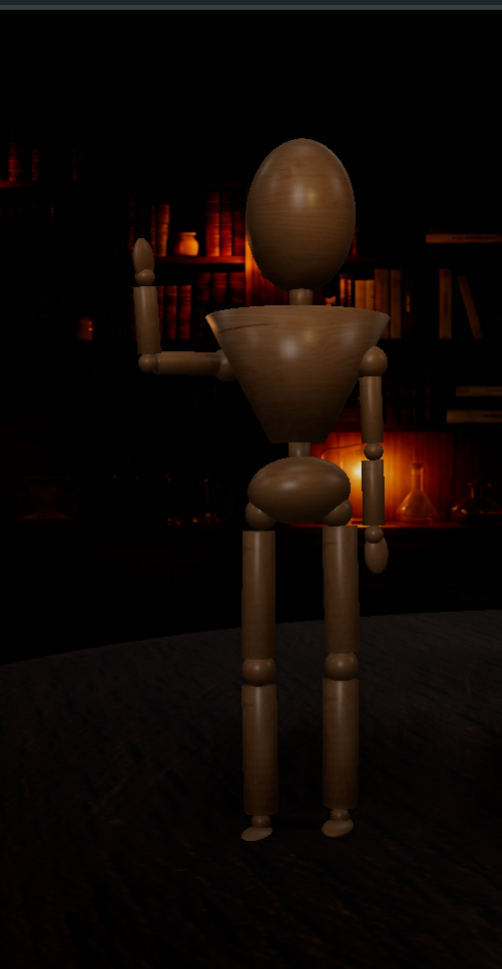
\includegraphics[width=0.4\textwidth]{dummy.png} 
    \caption{Dummy in action} 
    \label{fig:dummy} % Etichetta per richiamarla nel testo
\end{figure}

The idea of placing the portfolio inside a computer case emerged from a conversation with my roommate. I had told her that, as a child, I used to imagine computer motherboards as miniature cities: complex landscapes made of small buildings, streets and interconnected structures. Starting from this memory, she suggested transforming the interior of a computer case into the setting of the project. This idea became the foundation of \textit{Inside My System}, where the components of a computer are reinterpreted as parts of a small inhabited world.

\begin{figure}[h]
    \centering 
    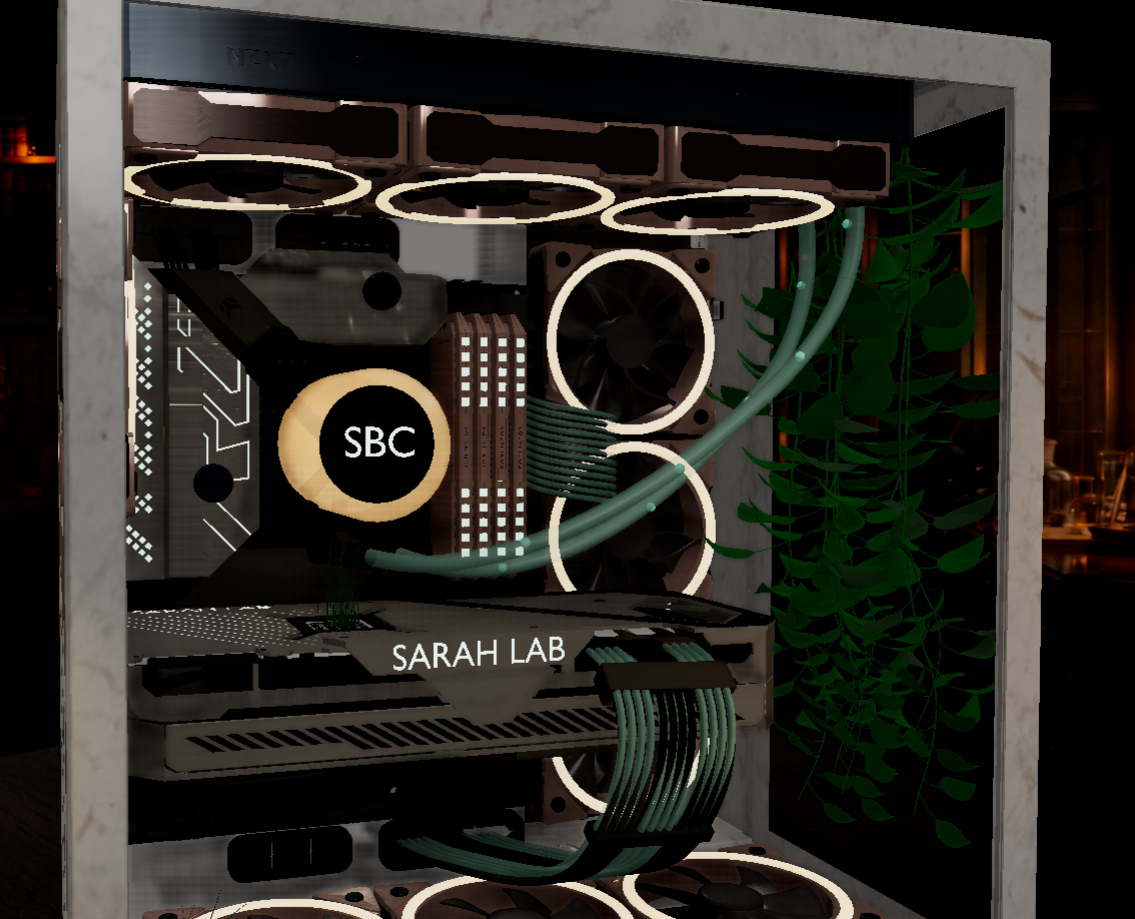
\includegraphics[width=0.8\textwidth]{case.png} 
    \caption{Case} 
    \label{fig:case} % Etichetta per richiamarla nel testo
\end{figure}

The title refers both to the physical computer system represented by the case and to the personal system of interests, experiences and skills contained within it. The user initially enters a dark environment and is invited to turn on a lamp. This action activates the computer and reveals the main scene, from which the different sections of the portfolio can be explored. Through lighting, camera movements, animated components and interactive labels, the project gradually introduces its contents while preserving the atmosphere of discovery that inspired its original concept.

\section{Libraries, Tools, and External Assets}

The project was developed using a limited set of third-party libraries, together with modelling, image-processing and version-control tools.
The application logic, interaction system and runtime animations were implemented specifically for \textit{Inside My System}, while external
software was used to support rendering, asset creation, interfacegraphics and production deployment.

\subsection{Third-Party Libraries}

Table~\ref{tab:third-party-libraries} lists the software dependencies
actively used by the final application.

\begin{table}[ht]
    \centering
    \small
    \setlength{\tabcolsep}{7pt}
    \renewcommand{\arraystretch}{1.25}

    \begin{tabularx}{\textwidth}{
        @{}
        >{\bfseries\raggedright\arraybackslash}p{0.20\textwidth}
        >{\centering\arraybackslash}p{0.14\textwidth}
        >{\raggedright\arraybackslash}X
        @{}
    }
        \toprule
        Library & Version & Purpose \\
        \midrule

        Three.js
        &
        0.184.0
        &
        Real-time WebGL rendering, scene-graph management, cameras,
        lights, materials, textures, raycasting and runtime geometry.
        Official Three.js addons are also used for GLB loading,
        camera controls and post-processing.
        \\

        GSAP
        &
        3.15.0
        &
        Smooth interpolation of the camera position and its target
        during transitions between the interactive portfolio sections.
        \\

        Simple Icons
        &
        16.25.0
        &
        SVG paths used for the contact icons displayed in the HTML
        portfolio interface.
        \\

        Vite
        &
        8.1.0
        &
        Development server, ES-module handling, production bundling and
        generation of the static build used for deployment.
        \\

        \bottomrule
    \end{tabularx}

    \caption{Third-party libraries used by the final application.}
    \label{tab:third-party-libraries}
\end{table}

Three.js is the main runtime dependency of the project. The application uses both its core scene-graph classes and several modules distributed
as official addons. \texttt{GLTFLoader} loads the complete scene from the binary glTF model, while \texttt{OrbitControls} provides damped
rotation, panning and zooming.

The post-processing pipeline is also implemented using official Three.js modules, including \texttt{EffectComposer}, \texttt{RenderPass}, \texttt{SSAOPass},
\texttt{UnrealBloomPass}, \texttt{ShaderPass} and \texttt{OutputPass}. These modules are therefore considered part of Three.js rather than separate third-party dependencies.

GSAP is used by the camera system to interpolate both the position of the perspective camera and the target observed by
\texttt{OrbitControls}. Updating the two properties simultaneously produces a controlled transition toward each portfolio component
without abrupt changes in orientation.
\subsection{Development and Authoring Tools}

The visual and technical assets were prepared through a combination of
three-dimensional modelling, scripting and version-control tools.

\begin{table}[ht]
    \centering
    \small
    \setlength{\tabcolsep}{7pt}
    \renewcommand{\arraystretch}{1.25}

    \begin{tabularx}{\textwidth}{
        @{}
        >{\bfseries\raggedright\arraybackslash}p{0.25\textwidth}
        >{\raggedright\arraybackslash}X
        @{}
    }
        \toprule
        Tool & Role in the project \\
        \midrule

        Blender
        &
        Creation, modification and assembly of the three-dimensional
        scene, preparation of object hierarchies, UV mapping and export
        of the final model in binary glTF format.
        \\

        Node.js and npm
        &
        Management of JavaScript dependencies and execution of the Vite
        development, build and preview commands.
        \\

        Python and Pillow
        &
        Image resizing, format conversion and compression performed by
        the texture-optimisation script.
        \\

        Git and GitHub
        &
        Version control, branch management, source-code hosting and
        publication of the final application.
        \\

        \bottomrule
    \end{tabularx}

    \caption{Development and asset-authoring tools.}
    \label{tab:development-tools}
\end{table}

A dedicated texture-optimisation workflow was created for the project.
A Node.js script specifies the required output size and compression quality for each texture map and invokes a Python routine based on Pillow. Different limits are applied according to the semantic role of each texture: colour and background images are generally preserved at
a higher resolution, while roughness and metalness maps can be reduced more aggressively.

The selected texture set was reduced from approximately
\(505\,\mathrm{MiB}\) to \(4.7\,\mathrm{MiB}\), corresponding to an overall file-size reduction of approximately \(99.1\%\). Further details about this process are provided in the performance-optimisationsection.

\subsection{External 3D Models}

The final scene is exported as a single
\texttt{portfolio\_case.glb} file, but it was assembled in Blender from
multiple original and external components. The external models were not
used as complete, unmodified scenes. Their geometry, scale, materials,
hierarchies and placement were adapted to the visual and interactive
requirements of the project.

The external models whose original listings could be recovered are
reported in Table~\ref{tab:identified-external-models}.

\begin{table}[ht]
    \centering
    \footnotesize
    \setlength{\tabcolsep}{5pt}
    \renewcommand{\arraystretch}{1.25}

    \begin{tabularx}{\textwidth}{
        @{}
        >{\bfseries\raggedright\arraybackslash}p{0.16\textwidth}
        >{\raggedright\arraybackslash}p{0.20\textwidth}
        >{\raggedright\arraybackslash}X
        >{\centering\arraybackslash}p{0.13\textwidth}
        @{}
    }
        \toprule
        Asset & Author and source & Use and modifications & License \\
        \midrule

        Table
        &
        \href{
        https://sketchfab.com/3d-models/table-1132fa2850a24917892733566bd68e74
        }{yryabchenko, Sketchfab}
        &
        Used as the supporting desk surface. Its scale, placement and
        material appearance were modified to match the composition and
        lighting of the final environment.
        &
        \href{
        https://creativecommons.org/licenses/by/4.0/
        }{CC BY 4.0}
        \\

        Gaming computer
        &
        \href{
        https://sketchfab.com/3d-models/gaming-computer-7cf383ddfe9047f89435b4fc2a6e1053
        }{Marcseus, Sketchfab}
        &
        Used as the starting point for the computer case and its
        internal hardware. The model was substantially reorganised and
        modified in Blender, with new materials, interactive targets,
        decorative elements and project-specific details.
        &
        \href{
        https://creativecommons.org/licenses/by/4.0/
        }{CC BY 4.0}
        \\

        \bottomrule
    \end{tabularx}

    \caption{External models with recovered source information.}
    \label{tab:identified-external-models}
\end{table}

Four additional Sketchfab models were incorporated into the final
Blender scene:

\begin{itemize}
    \item a desk-lamp model;
    \item a separate chain model used for the lamp interaction;
    \item a decorative plant model placed around the computer case;
    \item a second plant model used for additional foliage.
\end{itemize}

These assets were modified, renamed and merged into the final scene
before export. Their original Sketchfab listing metadata was not
preserved in the retained local files, and the corresponding author and
license information could not be recovered reliably. They are therefore
explicitly documented as external assets without assigning unsupported
attribution data.

The lamp was adapted to support the initial power-on interaction. Its
bulb and materials are controlled at runtime, while a separate invisible
click target is associated with the chain. The plant models were
rescaled, repositioned and duplicated; their materials are also adjusted
at runtime to preserve their readability in the dark environment.

\subsection{Textures and Visual Assets}

The main physically based texture sets were obtained from
\href{https://ambientcg.com/}{ambientCG}. The original asset identifiers
were retained in the material and folder names, allowing their sources
to be reconstructed from the project files.

All ambientCG assets are distributed under the Creative Commons
\href{https://creativecommons.org/publicdomain/zero/1.0/}{CC0 1.0}
licence. Attribution is not legally required, but the original resources
are listed in Table~\ref{tab:external-textures} for completeness.

\begin{table}[ht]
    \centering
    \small
    \setlength{\tabcolsep}{6pt}
    \renewcommand{\arraystretch}{1.22}

    \begin{tabularx}{\textwidth}{
        @{}
        >{\bfseries\raggedright\arraybackslash}p{0.21\textwidth}
        >{\raggedright\arraybackslash}X
        >{\centering\arraybackslash}p{0.13\textwidth}
        @{}
    }
        \toprule
        Texture set & Use in the project & License \\
        \midrule

        \href{https://ambientcg.com/view?id=Marble021}{Marble 021}
        &
        Marble surface applied to the computer-case structure.
        &
        CC0
        \\

        \href{https://ambientcg.com/view?id=Metal033}{Metal 033}
        &
        Metallic material used for the main fan surfaces.
        &
        CC0
        \\

        \href{https://ambientcg.com/view?id=Plastic004}{Plastic 004}
        &
        Rough plastic material applied to selected internal components.
        &
        CC0
        \\

        \href{https://ambientcg.com/view?id=Plastic013A}{Plastic 013 A}
        &
        Light plastic material used for the illuminated fan rings.
        &
        CC0
        \\

        \href{https://ambientcg.com/view?id=Metal043A}{Metal 043 A}
        &
        Metallic material used for fan outlines and selected memory
        components.
        &
        CC0
        \\

        \href{https://ambientcg.com/view?id=Metal045A}{Metal 045 A}
        &
        Metallic material applied to external CPU and GPU components.
        &
        CC0
        \\

        \bottomrule
    \end{tabularx}

    \caption{External PBR texture sets used by the application.}
    \label{tab:external-textures}
\end{table}

The texture system supports base-colour, normal, roughness and
metalness maps. Base-colour textures are interpreted in the sRGB colour
space, while the remaining maps are treated as data textures. The
optimised derivatives used by the final application are stored in
\texttt{public/textures\_optimized}.

The environmental background was created specifically for
\textit{Inside My System} and subsequently resized and compressed for
web delivery. It is rendered as the scene background and establishes
the nighttime library and studio atmosphere surrounding the
three-dimensional desk.

The contact interface uses SVG paths from Simple Icons for Gmail,
GitHub and Instagram. The LinkedIn SVG path is stored locally because
it is not exported by the installed version of the library.

\section{3D Assets and Scene Composition}

\subsection{Computer Case}

The computer case is the central three-dimensional asset of
\textit{Inside My System}. It is both the main setting of the portfolio
and the visual metaphor on which the project is based: the internal
components of a computer are reinterpreted as parts of a small personal
world, with each hardware element corresponding to a different section
of the portfolio.

The starting point was the external \textit{Gaming Computer} model
introduced in the previous section. However, the original asset was not
used as an unmodified prop. It was imported into Blender and
substantially reorganised to support the visual composition and the
interaction design of the project. The scale and position of the
components were adjusted, the case materials were replaced, and the
internal layout was adapted to make the individual elements clearly
visible from the main camera viewpoint.

Particular attention was given to the readability of the interior. The
CPU, GPU, RAM modules, cooling fans and cables had to remain visually
distinguishable even though they are contained within a relatively
compact space. These components were therefore arranged not only
according to their function as computer hardware, but also according to
their role as navigation elements. The CPU represents the About Me
section, the GPU gives access to Projects, the RAM modules contain the
Academic section, the fans represent Work Experience, and the cables
lead to Hobbies and Interests.

The original scene was extended with additional environmental and
narrative elements. Dummy was placed beside the case as the personal
representative of the author, while the lamp, plants and desk transform
the hardware model into a small inhabited environment. This composition
creates a contrast between the rigid geometry of the computer components
and the warmer, more organic forms surrounding them.

Although the final application loads the scene as a single binary glTF
file, the case remains internally divided into semantically meaningful
objects. Separate nodes are used for the major components, the fan
rotors, the illuminated parts and the invisible interaction targets.
This organisation allows the imported polygonal model to be treated as
a structured scene graph rather than as a single static mesh.

The naming convention introduced during the Blender preparation stage
is essential to this organisation. Interactive proxy objects use the
\texttt{CLICK\_} prefix, while the fan rotors use identifiers such as
\texttt{FAN\_ROT\_X}, \texttt{FAN\_ROT\_Y} and
\texttt{FAN\_ROT\_Z}. As a result, the JavaScript application can locate
specific objects after loading the model and associate them with the
appropriate animation or portfolio behaviour.

Some visual details are added or refined at runtime rather than being
stored exclusively in the GLB file. For example, the central CPU element
is completed with a circular illuminated ring, a dark internal disc and
an \texttt{SBC} label generated through a canvas texture. This approach
combines an authored Blender model with procedural Three.js elements,
allowing selected details to respond directly to the powered state of
the application.

The complete scene is exported as
\texttt{public/models/portfolio\_case.glb}. The glTF format was selected
because it preserves polygonal geometry, materials, transformations and
the parent--child hierarchy in a format designed for real-time
applications. Once loaded, the model can therefore retain the structural
information required for interaction and animation while being rendered
efficiently through Three.js.


\begin{figure}[ht]
    \centering

    \begin{minipage}[t]{0.48\textwidth}
        \centering
        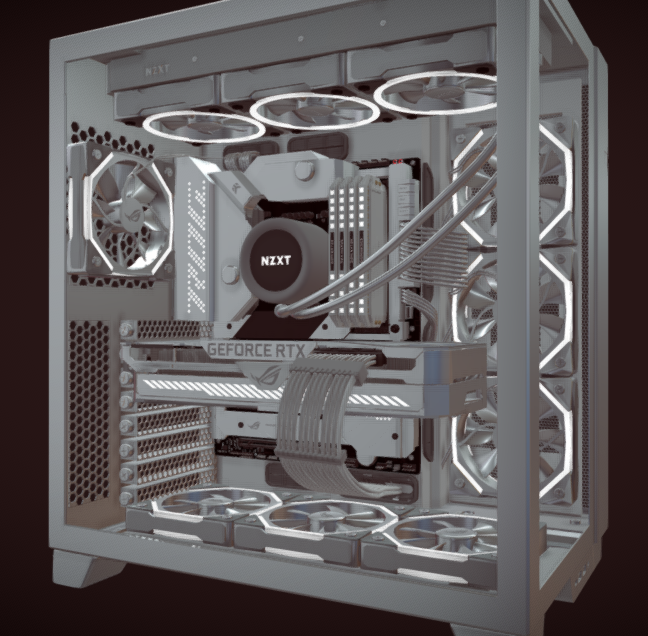
\includegraphics[width=\linewidth]{riginal-computer-model.png}
        \smallskip

        \textbf{(a)} Original external model
    \end{minipage}
    \hfill
    \begin{minipage}[t]{0.48\textwidth}
        \centering
        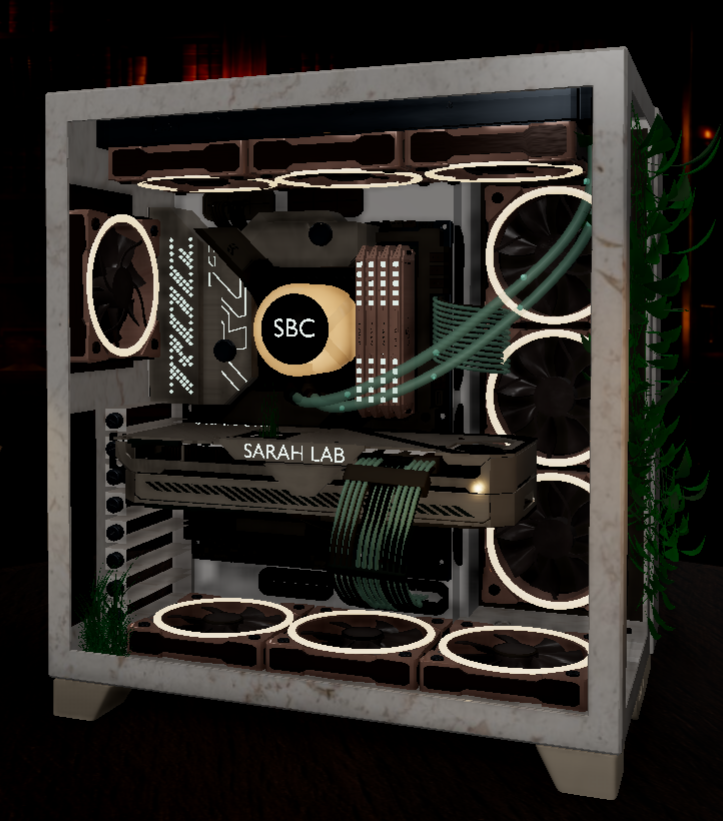
\includegraphics[width=\linewidth]{final-computer-case.png}
        \smallskip

        \textbf{(b)} Final scene after modification
    \end{minipage}

    \caption{The external computer model used as a starting point and
    its final reinterpretation in \textit{Inside My System}.}
    \label{fig:computer-case-comparison}
\end{figure}

\subsection{Dummy}

Dummy is the main character of \textit{Inside My System} and represents
the personal and creative dimension of the project. It is based on a
recurring figure from my illustrations, originally used to express
ideas, emotions and personal experiences without relying on a realistic
self-portrait. Its inclusion in the scene therefore creates a direct
connection between my illustration practice and the interactive
portfolio.

While the computer case represents the technical structure of the
project, Dummy introduces a more human element into the environment. It
is positioned beside the case as a small inhabitant of the system and
acts as the visual representation of the author. The contrast between
the wooden mannequin and the electronic components reinforces the
combination of illustration and engineering on which the project is
based.

The three-dimensional version of Dummy was prepared in Blender as a
collection of separate rigid parts. The body, neck, head, arms, forearms
and hands remain distinct objects instead of being merged into a single
mesh. This separation is necessary because each component must preserve
an independent local transformation during the runtime animations.

Dummy is not animated through a skeletal rig or through animation clips
exported from Blender. Instead, its movements are produced directly in
JavaScript by modifying the transformations of the individual objects.
The Blender model therefore provides the geometry and the initial pose,
while the final animation behaviour is implemented by the application.

The model is organised under a common root node named
\texttt{Dummy\_root}. Its main movable components use semantic names
such as \texttt{Dummy\_body}, \texttt{Dummy\_neck} and
\texttt{Dummy\_head}. Additional anchor objects identify the positions
of the right shoulder, elbow and wrist. These anchors allow the
application to construct an articulated parent--child hierarchy after
the GLB scene has been loaded.

This organisation follows the principle of hierarchical modelling. A
transformation applied to a parent node is inherited by all of its
descendants. For example, rotating the shoulder affects the complete
arm, while rotating the elbow modifies only the forearm and hand.
Similarly, the wrist transformation affects the hand without changing
the upper parts of the limb. The model can therefore produce articulated
motion through a sequence of local transformations rather than by
manually updating every mesh in world coordinates.

Two principal behaviours were designed for Dummy. During the idle state,
its body, neck and head gradually follow the position of the user's
pointer. The head reacts with the largest rotation, while the neck and
body use progressively smaller movements. This distribution creates the
impression that the character is observing the visitor without requiring
complex facial animation.

When Dummy is selected, it performs a short greeting animation. The
right arm is raised through the shoulder joint, the forearm is bent at
the elbow and a smooth oscillation produces the waving movement. The
wrist also receives a smaller secondary rotation, making the gesture
appear less rigid. At the end of the animation, all articulated parts
return to their original local rotations.

A dedicated invisible object named \texttt{CLICK\_DUMMY} is used as the
interaction target. Keeping this proxy separate from the visible
geometry simplifies raycasting and avoids depending on the detailed
shape of the mannequin. Clicking the target moves the camera towards
Dummy, opens its portfolio content and activates the greeting animation.

The visual material of the mannequin is configured separately from the
other scene components. Its physically based material uses a colour
map, a normal map and a roughness map, preserving the appearance of a
wooden drawing mannequin while remaining consistent with the lighting
of the surrounding environment.

\begin{figure}[ht]
    \centering

    \begin{minipage}[t]{0.30\textwidth}
        \centering
        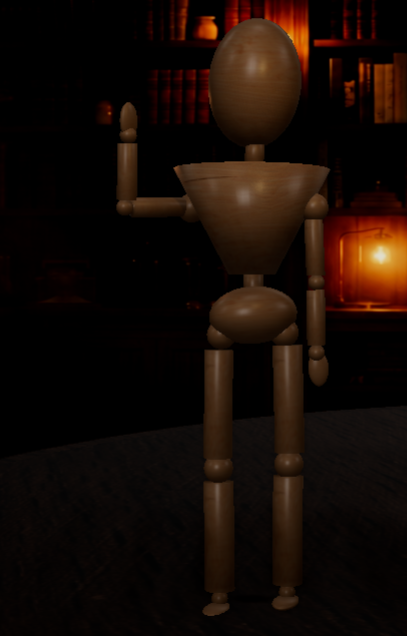
\includegraphics[width=\linewidth]{dummy-final-scene.png}
        \smallskip

        \textbf{(a)} Dummy inside the final scene
    \end{minipage}
    \hfill
    \begin{minipage}[t]{0.50\textwidth}
        \centering
        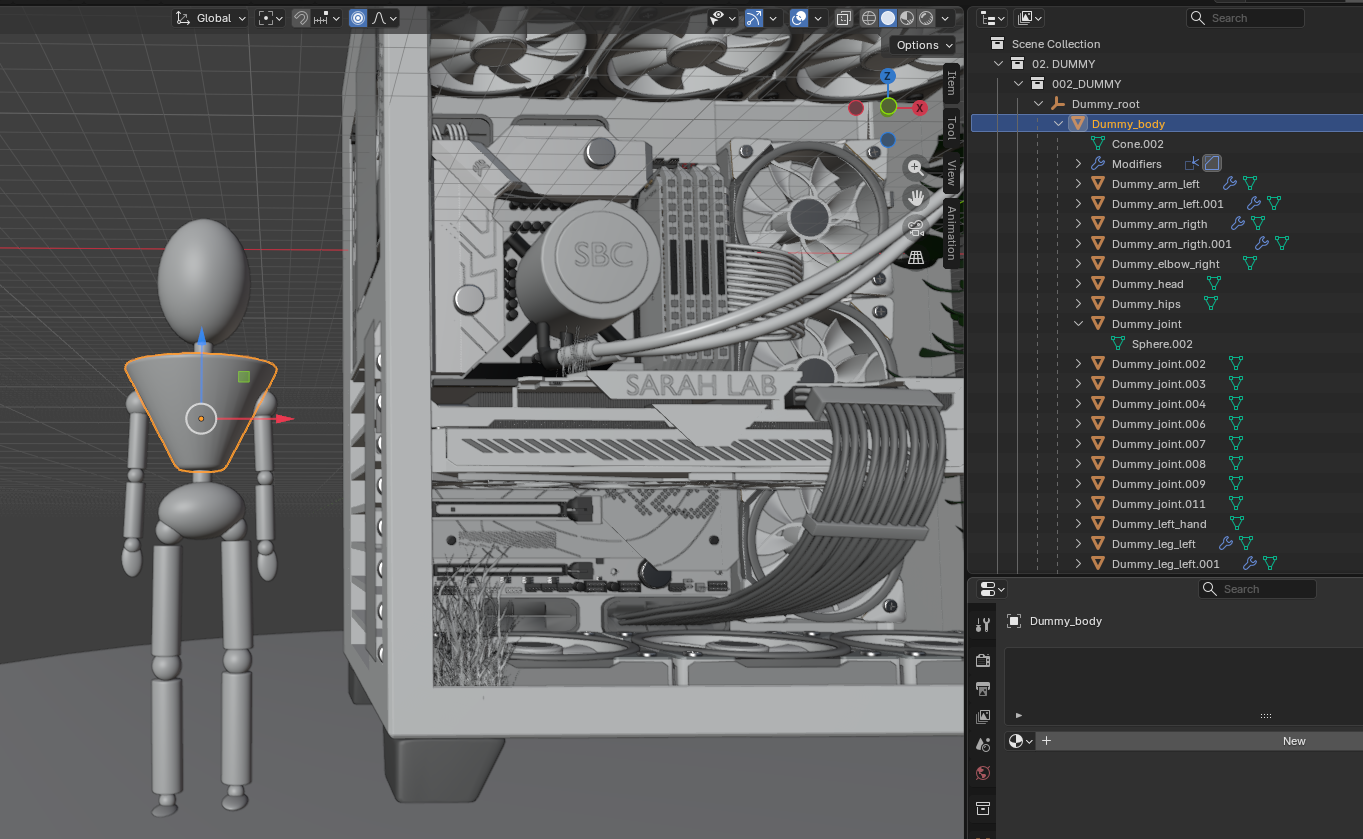
\includegraphics[width=\linewidth]{dummy-hierarchy.png}
        \smallskip

        \textbf{(b)} Object hierarchy prepared for animation
    \end{minipage}

    \caption{Dummy as it appears in the final environment and the
    separate objects used to construct its articulated hierarchy.}
    \label{fig:dummy-model}
\end{figure}

\subsection{Lamp and Desk Environment}

The computer case is placed within a small desk environment designed to
give the scene a warmer and more personal identity. The surrounding
objects are not only decorative: they establish the initial visual
composition, support the lighting design and guide the user towards the
first interaction.

The table provides the common supporting surface for the complete scene.
The computer case, Dummy and the desk lamp are arranged on top of it so
that they can be perceived as parts of the same physical environment.
Its broad surface also receives the shadows and pools of light generated
by the local light sources, helping the separate assets appear visually
grounded rather than floating independently in space.

The original table model was modified in Blender to match the scale and
composition of the project. Its material was replaced with a physically
based surface using colour, normal and roughness maps. Compared with the
harder and more reflective materials of the computer case, the table was
given a relatively high roughness so that it produces broader highlights
and contributes to the restrained nighttime atmosphere.

The desk lamp is positioned on the opposite side of the composition from
the computer case. This creates a visual balance between the warm light
source and the illuminated hardware. More importantly, the lamp acts as
the entry point of the interactive experience. The application initially
opens in a dark state, with the camera directed towards the lamp and its
hanging chain. Pulling the chain turns on the environment and reveals the
main portfolio scene.

The lamp and the chain originated as separate external models and were
combined during the preparation of the Blender scene. The lamp retains
distinct objects for its body, shade and bulb, allowing the bulb and
shade materials to be controlled independently at runtime. The visible
chain is also kept as a separate object, while an additional invisible
proxy named \texttt{CLICK\_CHAIN} provides a larger and more reliable
raycasting target.

The separation between visible geometry and interaction geometry is
particularly useful for thin objects. Using the individual chain links
as raycasting targets would require the pointer ray to intersect a very
small surface. The dedicated proxy preserves the appearance of the
original model while making the interaction easier to discover and
activate.

The chain is also prepared for a programmatic pull animation. Its root
object and the invisible click target move together along their local
downward direction. A small oscillation is applied during the movement,
while the vertices of the visible chain receive a progressively stronger
deformation towards the free end. This produces a more flexible response
than translating the complete model as a rigid object.

Two modified plant assets were added around the case to introduce
organic shapes into an environment dominated by mechanical components.
Their curved leaves and irregular silhouettes soften the geometry of the
computer hardware and reinforce the concept of the case as a small
inhabited world. The plants were rescaled, repositioned and duplicated
in Blender to fit the available space without covering the interactive
components.

Because the original plant materials appeared excessively dark under the
nighttime lighting, their appearance is corrected after the GLB model is
loaded. Plant-like meshes are identified through their object hierarchy
and assigned cloned materials with reduced metalness, increased
roughness and a restrained green tint. This adjustment improves their
readability without introducing an additional light source solely for
the foliage.

The three-dimensional scene is surrounded by a blurred nighttime
background representing a quiet library and creative studio. The image
was created specifically for the project and is visually richer near the
sides while remaining less contrasted behind the main case. This
composition prevents the background from competing with the interactive
objects and supports the depth separation between the foreground models
and the surrounding room.

The environment therefore combines three different visual categories:
the rigid technical geometry of the computer, the articulated figure of
Dummy and the warmer domestic elements of the desk. The lamp provides
the principal motivated light source, the table establishes a shared
physical support, and the plants and background connect the scene to the
personal and illustrative identity of the portfolio.


\begin{figure}[ht]
    \centering
    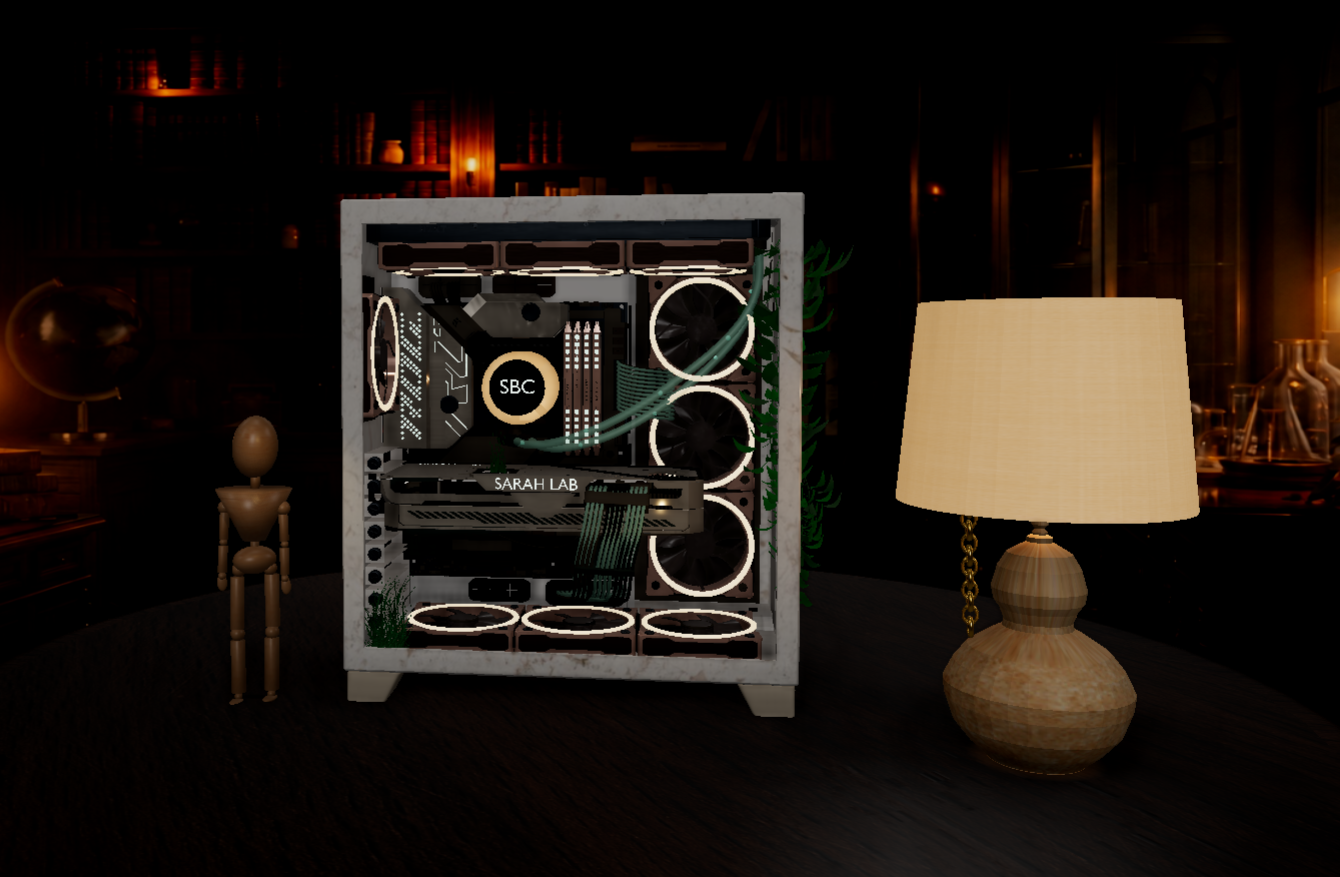
\includegraphics[width=0.92\textwidth]
        {desk-environment.png}

    \caption{The final desk environment, including the computer case,
    Dummy, the interactive lamp, the supporting table and the decorative
    vegetation.}
    \label{fig:desk-environment}
\end{figure}

\subsection{Scene Hierarchy and GLB Organisation}

The complete three-dimensional environment is exported from Blender as
a single binary glTF file named
\texttt{portfolio\_case.glb}. Although the application loads one file,
the scene is not represented as a single merged mesh. The GLB preserves
a hierarchy of named objects corresponding to the main assets,
individual hardware components, movable parts and interaction proxies.

This organisation allows the imported scene to be managed as a scene
graph. Every node stores a local transformation relative to its parent,
and the corresponding world transformation is obtained by composing the
transformations along the hierarchy. Consequently, related objects can
be moved or rotated as groups while preserving the relative placement
of their descendants.

The hierarchy was prepared primarily in Blender. The desk environment
contains separate roots for the table, computer case, Dummy, lamp,
chain and decorative vegetation. Within the computer case, the CPU,
GPU, RAM modules, cooling tubes, fan structures and illuminated
components remain identifiable as independent nodes. This subdivision
is required because different components participate in different
runtime behaviours.

Semantic object names provide the connection between the authored model
and the JavaScript application. After loading the GLB, the program
searches the hierarchy by name and assigns each recognised object a
specific role. For example, \texttt{Dummy\_root} identifies the
articulated mannequin, \texttt{LAMPADINA\_4} identifies the lamp bulb,
and \texttt{CPU\_CENTRAL\_RING} identifies the illuminated ring around
the central processor element.

Objects whose names begin with \texttt{CLICK\_} are invisible
interaction proxies. They are deliberately separated from the visible
meshes and placed on a dedicated raycasting layer. The principal targets
are:

\begin{itemize}
    \item \texttt{CLICK\_DUMMY}, associated with the introductory panel;
    \item \texttt{CLICK\_CPU}, associated with the About Me section;
    \item \texttt{CLICK\_GPU}, associated with Projects;
    \item \texttt{CLICK\_RAM}, associated with the Academic section;
    \item \texttt{CLICK\_FANS}, associated with Work Experience;
    \item \texttt{CLICK\_CABLES}, associated with Hobbies and Interests;
    \item \texttt{CLICK\_CHAIN}, associated with the power interaction.
\end{itemize}

Using proxy geometry provides two advantages. First, the clickable area
can be larger and simpler than the corresponding visible object, making
the interaction more reliable. Second, the appearance of the model can
be modified without changing the interaction logic, as long as the
semantic proxy names are preserved.

A similar naming convention is used for animated components. Fan rotors
are identified through names such as \texttt{FAN\_ROT\_X},
\texttt{FAN\_ROT\_Y\_1} and \texttt{FAN\_ROT\_Z\_1}. Each recognised
rotor is associated with a local rotation axis and a slightly different
speed multiplier, creating controlled variation between the fans. The
visible lamp chain is instead located through its normalised object name
and connected to the chain animator together with
\texttt{CLICK\_CHAIN}.

Not every node used by the final scene is stored directly in the GLB.
Some elements are generated or reorganised after loading. The CPU core
decoration, its label and part of its illuminated ring are created
procedurally in Three.js. Dummy's shoulder, elbow and wrist pivots are
also constructed at runtime and inserted into the imported hierarchy.
This hybrid approach keeps the visual composition editable in Blender
while allowing the application to create structures whose behaviour is
defined entirely in JavaScript.

The loading process therefore consists of several stages. First,
\texttt{GLTFLoader} reconstructs the scene graph contained in the GLB.
The application then assigns project-specific materials, secures the
rendering properties of imported materials, registers the interaction
targets and locates the objects required by the animation systems.
Finally, procedural details, lighting controllers and runtime pivots are
added to the imported model.

A simplified representation of the final hierarchy is shown below:

\begin{verbatim} [center]
portfolio_case.glb
|
+-- Table
+-- Computer case
|   +-- CPU
|   |   +-- CPU_CENTRAL_RING
|   +-- GPU
|   +-- RAM
|   +-- Cooling tubes
|   +-- Fans
|       +-- FAN_ROT_X
|       +-- FAN_ROT_Y_1 ...
|       +-- FAN_ROT_Z_1 ...
|
+-- Dummy_root
|   +-- Dummy_body
|   +-- Dummy_neck
|   +-- Dummy_head
|   +-- Right arm components
|
+-- Lamp
|   +-- LAMPADINA_4
|   +-- Chain
|
+-- Decorative plants
|
+-- Interaction proxies
    +-- CLICK_DUMMY
    +-- CLICK_CPU
    +-- CLICK_GPU
    +-- CLICK_RAM
    +-- CLICK_FANS
    +-- CLICK_CABLES
    +-- CLICK_CHAIN
\end{verbatim}

This structure makes the GLB more than a container for polygonal
geometry. It acts as the shared interface between the Blender scene and
the runtime application: geometry and initial transformations are
authored visually, while names and hierarchy expose the elements that
must be controlled through code.

\section{Technical Description}

\subsection{Software Architecture}

The application is organised as a set of JavaScript ES modules divided
according to their runtime responsibility. The architecture is not a
strict inheritance hierarchy: it is more accurately described as a
composition of controllers coordinated by a central application object.

The entry point is \texttt{main.js}. It imports the global stylesheet,
selects the WebGL canvas and creates an instance of the
\texttt{Experience} class. During development, the same instance is
also exposed through a browser variable for diagnostic and camera
calibration operations.

\texttt{Experience} is the central application coordinator. It follows
a singleton-like pattern, ensuring that only one shared scene, camera,
renderer and interaction state are created. Its constructor initialises
the core services in the following order:

\begin{enumerate}
    \item the Three.js scene;
    \item the global interaction-state manager;
    \item the viewport-size and timing utilities;
    \item the camera controller;
    \item the renderer;
    \item the optional debugging and guidance systems;
    \item the world;
    \item the raycasting and portfolio-interface controller.
\end{enumerate}

The renderer is created before the world so that the environment and
model-loading modules can access an already configured WebGL renderer.
If a WebGL context cannot be created, the three-dimensional world and
the interaction controller are not initialised, and the application
displays a fallback message instead.

\subsubsection{Core application layer}

The core layer contains the modules that coordinate the complete
execution of the application.

\begin{table}[ht]
    \centering
    \small
    \setlength{\tabcolsep}{7pt}
    \renewcommand{\arraystretch}{1.22}

    \begin{tabularx}{\textwidth}{
        @{}
        >{\bfseries\raggedright\arraybackslash}p{0.26\textwidth}
        >{\raggedright\arraybackslash}X
        @{}
    }
        \toprule
        Module & Responsibility \\
        \midrule

        \texttt{Experience}
        &
        Creates and coordinates the shared scene, runtime services,
        update loop and high-level application events.
        \\

        \texttt{Sizes}
        &
        Stores the viewport dimensions and pixel ratio and emits resize
        notifications.
        \\

        \texttt{Time}
        &
        Runs the \texttt{requestAnimationFrame} loop and calculates
        elapsed and per-frame time.
        \\

        \texttt{Camera}
        &
        Owns the perspective camera, \texttt{OrbitControls} and GSAP
        transitions between predefined viewpoints.
        \\

        \texttt{Renderer}
        &
        Owns the WebGL renderer, shadow configuration, tone mapping and
        post-processing composers.
        \\

        \texttt{InteractionStateManager}
        &
        Stores the global interaction state and coordinates transition
        locks.
        \\

        \bottomrule
    \end{tabularx}

    \caption{Core runtime modules.}
    \label{tab:core-runtime-modules}
\end{table}

The main update loop is owned by \texttt{Experience}. On each animation
frame, it updates the camera controls, delegates scene updates to the
world, updates the interaction controller and finally renders the
frame. The world therefore updates all model animations before the
renderer processes the current scene state.

\subsubsection{World and scene-content layer}

The \texttt{World} class is intentionally small. It creates only two
direct components:

\begin{itemize}
    \item \texttt{Environment};
    \item \texttt{PortfolioModel}.
\end{itemize}

\texttt{Environment} configures the scene background, the generated
environment map and the general illumination. It also exposes a power
transition method through which the ambient, hemisphere, directional
and supporting lights change intensity when the system is activated.

\texttt{PortfolioModel} is the principal scene-content controller. It
loads \texttt{portfolio\_case.glb} and coordinates the modules that act
on the imported model. Its responsibilities include:

\begin{itemize}
    \item applying and enhancing materials;
    \item registering the invisible interaction proxies;
    \item identifying animated objects in the GLB hierarchy;
    \item constructing procedural CPU details;
    \item configuring shadows;
    \item initialising the power and lighting systems;
    \item creating and updating the animation controllers.
\end{itemize}

The model-related dependencies created or coordinated by
\texttt{PortfolioModel} are shown in
Table~\ref{tab:portfolio-model-components}.

\begin{table}[ht]
    \centering
    \small
    \setlength{\tabcolsep}{6pt}
    \renewcommand{\arraystretch}{1.2}

    \begin{tabularx}{\textwidth}{
        @{}
        >{\bfseries\raggedright\arraybackslash}p{0.29\textwidth}
        >{\raggedright\arraybackslash}X
        @{}
    }
        \toprule
        Component & Role \\
        \midrule

        \texttt{ApplyingTexture}
        &
        Loads and assigns the optimised texture maps to recognised
        model materials.
        \\

        \texttt{MaterialEnhancements}
        &
        Applies additional project-specific material corrections.
        \\

        \texttt{PlantMaterialTint}
        &
        Adjusts plant-like materials for the nighttime environment.
        \\

        \texttt{CozyLedMaterials}
        &
        Configures and animates the emissive LED materials used by the
        computer case.
        \\

        \texttt{DummyAnimator}
        &
        Controls pointer-following behaviour and the greeting animation
        of Dummy.
        \\

        \texttt{AnimatorChain}
        &
        Animates the visible lamp chain and its interaction proxy.
        \\

        \texttt{FanAnimator}
        &
        Rotates the recognised fan objects around their configured local
        axes.
        \\

        \texttt{TubeFlowAnimator}
        &
        Generates and animates the particles moving through the cooling
        tubes.
        \\

        \texttt{PowerExperience}
        &
        Coordinates the powered state, lamp emission, case LEDs, fans,
        renderer exposure and environment intensities.
        \\

        \texttt{ExtraLight}
        &
        Creates the additional warm lamp-light rig and its local
        shadow-casting source.
        \\

        \bottomrule
    \end{tabularx}

    \caption{Components coordinated by \texttt{PortfolioModel}.}
    \label{tab:portfolio-model-components}
\end{table}

This makes \texttt{PortfolioModel} the main integration point between
the authored GLB scene and the runtime behaviour implemented in
JavaScript.

\subsubsection{Interaction and interface layer}

The interaction layer is centred on
\texttt{RaycasterController}. This module owns a Three.js raycaster,
tracks the pointer position and queries only the dedicated layer
containing the \texttt{CLICK\_} proxy objects.

\texttt{RaycasterController} also creates the
\texttt{SectionPanel}. The panel is therefore not a child of
\texttt{World} or \texttt{PortfolioModel}: it belongs to the
interaction and DOM-interface layer. When a valid target is selected,
the controller coordinates several separate modules:

\begin{itemize}
    \item it queries \texttt{InteractionStateManager};
    \item it opens the appropriate \texttt{SectionPanel} content;
    \item it starts a transition through \texttt{Camera};
    \item it can activate \texttt{PowerExperience};
    \item it can trigger \texttt{AnimatorChain} or
    \texttt{DummyAnimator}.
\end{itemize}

The portfolio data itself is stored separately in
\texttt{content/portfolioSections.js}. The
\texttt{SectionPanel} reads this data and creates the corresponding DOM
content, including regular text pages, academic tabs, project views,
work-experience entries and contact links.

The \texttt{GuidanceOverlay} is created directly by
\texttt{Experience}. It displays the initial instruction, the main
exploration message and context-dependent reminders after periods of
inactivity. Its visibility depends on the loading state, the current
interaction state, camera transitions and whether a portfolio panel is
open.

\subsubsection{Development utilities}

\texttt{DebugUtils} is also created directly by
\texttt{Experience}, but only becomes active when the
\texttt{debug=1} URL parameter is present. It receives references to
the canvas, camera controller, scene and interaction manager.

After the GLB is loaded, \texttt{PortfolioModel} passes the imported
scene to \texttt{DebugUtils}. The utility can then inspect mesh
hierarchies, material properties, texture dimensions, approximate
triangle counts and camera presets without placing debugging behaviour
inside the production controllers.

\subsubsection{Runtime composition}

The following diagram represents object creation and ownership more
accurately than a simple folder hierarchy:

\begin{verbatim}
main.js
|
`-- Experience
    |
    |-- THREE.Scene
    |-- InteractionStateManager
    |-- Sizes
    |-- Time
    |-- Camera
    |   `-- OrbitControls
    |
    |-- Renderer
    |   |-- WebGLRenderer
    |   |-- Bloom composer
    |   `-- Final composer
    |
    |-- GuidanceOverlay
    |-- DebugUtils
    |
    |-- World
    |   |-- Environment
    |   `-- PortfolioModel
    |       |-- ApplyingTexture
    |       |-- MaterialEnhancements
    |       |-- PlantMaterialTint
    |       |-- CozyLedMaterials
    |       |-- DummyAnimator
    |       |-- AnimatorChain
    |       |-- FanAnimator
    |       |-- TubeFlowAnimator
    |       |-- PowerExperience
    |       `-- ExtraLight
    |
    `-- RaycasterController
        `-- SectionPanel
            |-- portfolioSections
            `-- contactIcons
\end{verbatim}

The diagram describes ownership and construction, but communication is
not restricted to downward calls. The modules share references supplied
through \texttt{Experience}. For example,
\texttt{RaycasterController} communicates with the camera, world,
interaction manager and guidance overlay, while
\texttt{PowerExperience} modifies the environment, renderer, LED
controller and fan animator.

The resulting architecture combines composition, shared services and
event-based communication. It separates scene rendering, model
configuration, interaction, animation and DOM content while preserving
a single coordinated runtime state.

\subsection{Hierarchical Model: Dummy}

Dummy is the main hierarchical model of the project. Its geometry is
stored in the GLB file as a set of separate rigid parts rather than as a
single merged mesh. The principal objects include the body, neck, head,
upper arms, forearms and hands, together with anchor objects identifying
the shoulder, elbow and wrist positions.

The runtime application locates the complete character through the
\texttt{Dummy\_root} node and traverses its descendants to create a map
between semantic names and Three.js objects. The body, neck and head can
therefore be accessed directly through names such as
\texttt{Dummy\_body}, \texttt{Dummy\_neck} and
\texttt{Dummy\_head}.

The imported hierarchy is extended at runtime with three additional
pivot groups:

\begin{itemize}
    \item \texttt{rightShoulderPivot};
    \item \texttt{rightElbowPivot};
    \item \texttt{rightWristPivot}.
\end{itemize}

Each pivot is positioned at the world-space location of the
corresponding anchor and then converted into the local coordinate system
of its parent. The related limb component is attached to the new pivot
while preserving its world transformation.

A simplified representation of the runtime hierarchy is shown below:

\begin{verbatim}
Dummy_root
|
`-- Dummy_body
    |
    |-- Dummy_neck
    |   `-- Dummy_head
    |
    `-- rightShoulderPivot
        |-- Dummy_arm_right
        |
        `-- rightElbowPivot
            |-- Dummy_arm_right001
            |
            `-- rightWristPivot
                `-- Dummy_right_hand
\end{verbatim}

In a hierarchical model, the world transformation of a node is obtained
by composing its local matrix with the world matrix of its parent:

\[
\mathbf{M}^{\mathrm{world}}_{i}
=
\mathbf{M}^{\mathrm{world}}_{\mathrm{parent}(i)}
\mathbf{M}^{\mathrm{local}}_{i}.
\]

Consequently, a rotation of the shoulder pivot affects the upper arm,
forearm and hand. A rotation of the elbow affects only the forearm and
hand, while the wrist controls only the final hand component. This
propagation of transformations makes articulated motion possible
without computing independent world-space coordinates for every mesh.

The use of runtime pivots was preferred to a skeletal animation exported
from Blender. The geometry and initial pose are authored in the modelling
environment, while the animation logic remains completely visible and
controllable in JavaScript. This also satisfies the requirement that the
project animations be implemented programmatically rather than imported
as precomputed clips.


\subsection{Model Loading and Runtime Configuration}

The complete scene is loaded through \texttt{GLTFLoader} from
\texttt{models/portfolio\_case.glb}. The URL is constructed using
\texttt{import.meta.env.BASE\_URL}, ensuring that the same code works
both from the root of the local development server and from the
repository subdirectory used by GitHub Pages.

Before the GLB becomes available, \texttt{PortfolioModel} creates a
small placeholder scene containing a simplified computer case, a glass
panel and a capsule representing Dummy. The placeholder provides
immediate visual feedback during loading and remains visible if the GLB
cannot be retrieved.

Once loading succeeds, the imported scene passes through a sequence of
configuration stages:

\begin{enumerate}
    \item optimised textures and project-specific materials are assigned;
    \item selected CPU names and materials are normalised;
    \item the procedural CPU core decoration is created;
    \item shared GLB materials are cloned before runtime modification;
    \item emissive LED roles are identified and configured;
    \item the imported scene is added to the Three.js scene;
    \item Dummy, the chain, fan rotors and interaction proxies are located;
    \item material enhancements and plant corrections are applied;
    \item animation, power and lighting controllers are instantiated;
    \item the placeholder and loading interface are hidden.
\end{enumerate}

Cloning imported materials is important because multiple GLB meshes may
refer to the same material instance. Without cloning, changing
transparency, emission or depth-writing properties on one mesh could
unintentionally affect another object using the same source material.

Several elements are generated directly in Three.js after loading. The
central CPU receives a group containing a circular disc, a torus-shaped
light ring and an \texttt{SBC} label. The label is drawn on an HTML
canvas and transferred to the GPU through a
\texttt{CanvasTexture}. A procedural contact shadow is also placed
under Dummy using the bounding boxes of the character and the table.

The project therefore uses a hybrid asset workflow. Blender provides the
polygonal scene, the initial transformations and the object naming
scheme, while JavaScript adds the structures whose appearance or
behaviour must react dynamically to the application state.

\begin{figure}[H]
    \centering
    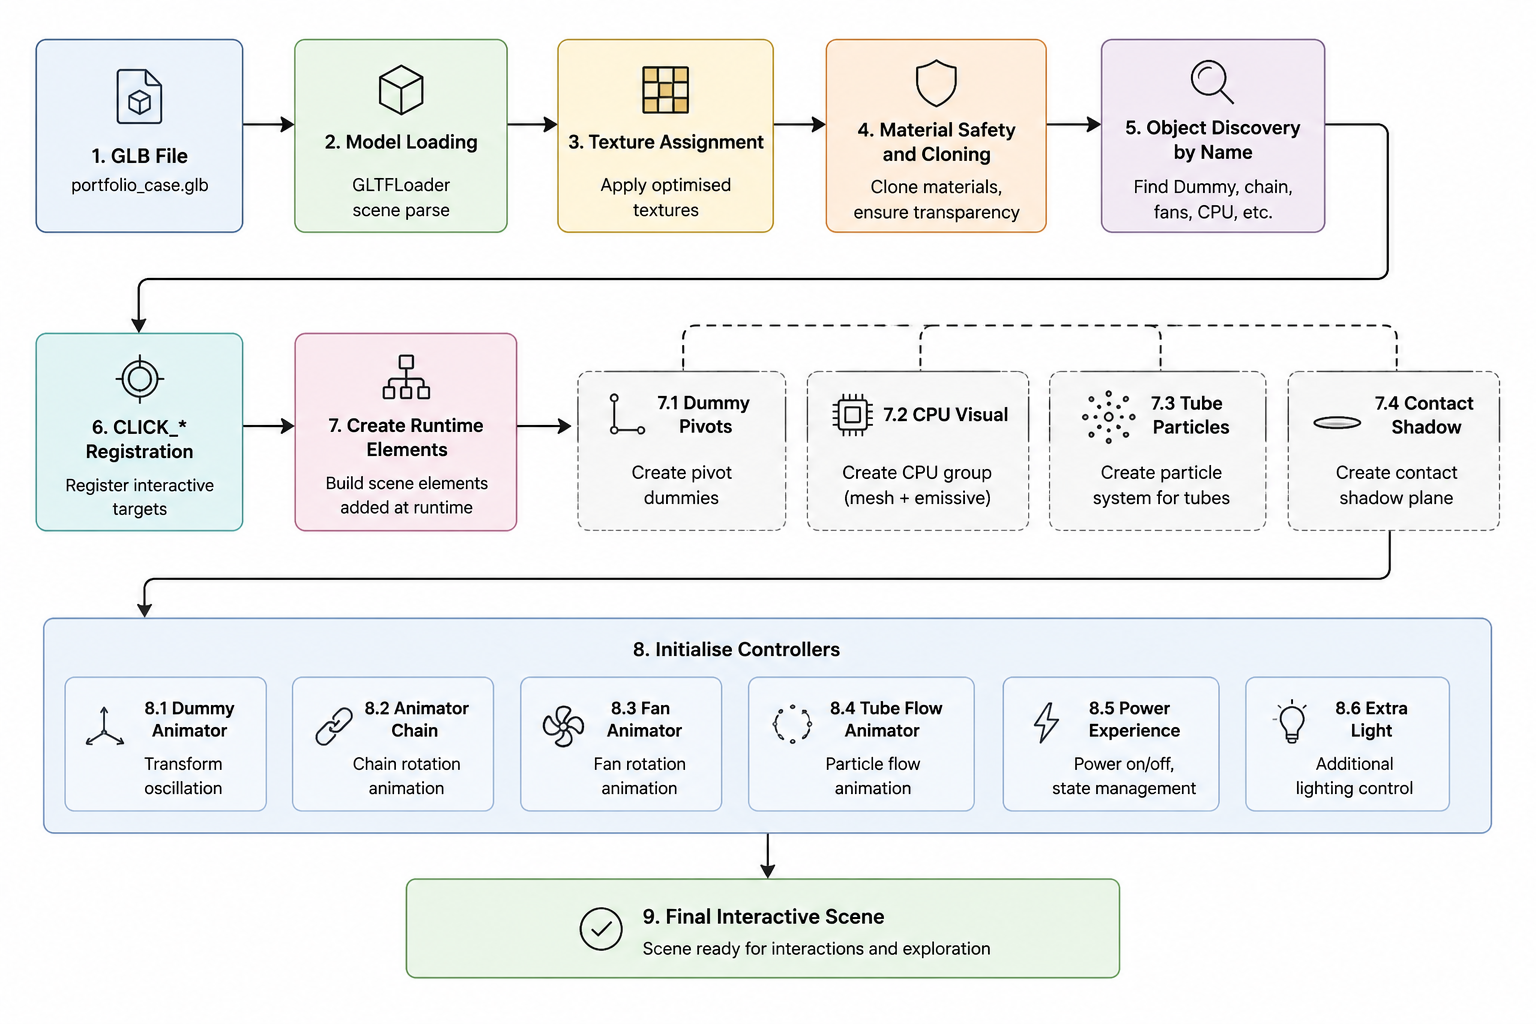
\includegraphics[width=0.85\textwidth]
        {model-loading-pipeline.png}
    \caption{Runtime processing stages applied to the imported GLB scene.}
    \label{fig:model-loading-pipeline}
\end{figure}


\subsection{Materials and Textures}

The visible objects are primarily rendered with
\texttt{MeshStandardMaterial}, which implements a physically based
metallic--roughness workflow. In this model, the visual response of a
surface depends on the incoming illumination, the base colour and the
material parameters controlling microscopic roughness and metallic
behaviour.

The texture system distinguishes between colour textures and data
textures. Base-colour maps are interpreted in the sRGB colour space,
because their stored values represent perceptual colours. Normal,
roughness and metalness maps remain linear data and are therefore not
assigned an sRGB colour-space transformation.

\begin{table}[ht]
    \centering
    \small
    \setlength{\tabcolsep}{7pt}
    \renewcommand{\arraystretch}{1.22}

    \begin{tabularx}{\textwidth}{
        @{}
        >{\bfseries\raggedright\arraybackslash}p{0.22\textwidth}
        >{\raggedright\arraybackslash}X
        @{}
    }
        \toprule
        Texture map & Function \\
        \midrule

        Base colour
        &
        Defines the visible diffuse colour of the surface and is decoded
        from the sRGB colour space.
        \\

        Normal map
        &
        Perturbs the interpolated surface normal, adding small-scale
        detail without increasing geometric complexity.
        \\

        Roughness map
        &
        Controls the spread of reflected highlights across the surface.
        Higher values produce broader and less defined reflections.
        \\

        Metalness map
        &
        Distinguishes dielectric regions from metallic regions and
        modifies the balance between diffuse and specular reflection.
        \\

        \bottomrule
    \end{tabularx}

    \caption{Principal PBR texture maps used by the application.}
    \label{tab:pbr-map-functions}
\end{table}

Since the texture coordinates originate from Blender and are exported
through glTF, loaded maps use \texttt{flipY = false}. This prevents the
vertical inversion that would otherwise occur when applying regular
Three.js texture conventions to glTF UV coordinates.

Material assignment is based on semantic information contained in
object names, material names and ancestor names. Recognised categories
include the case, table, Dummy, memory modules, cooling tubes, fans,
fan rings, external CPU and GPU components, metallic hardware and case
feet. The selected role is also stored in \texttt{userData}, allowing
later systems to identify materials without repeating the original
classification process.

Meshes that do not match a specific category receive a deterministic
fallback material selected from a restrained palette of graphite, warm
grey, taupe, bronze and desaturated green. The deterministic selection
keeps the final appearance stable between executions.

Transparency requires additional care because transparent fragments are
normally sorted and blended after opaque geometry. The project preserves
transparency only for explicitly identified glass, tube and label
materials. Glass and cooling tubes keep depth testing enabled but disable
depth writing, preventing them from incorrectly hiding opaque objects
rendered afterwards. Other imported materials are forced to be opaque
and use normal blending.

Many imported components consist of thin or disconnected surfaces with
inconsistent winding. To avoid missing faces when viewed from different
angles, their materials are rendered using
\texttt{THREE.DoubleSide}. This increases fragment processing compared
with back-face culling, but provides a more reliable result for the
retained external geometry.

The plants require a separate correction because their original
materials appear too dark under the nighttime lighting. Plant meshes are
recognised through names such as \texttt{plant}, \texttt{vine},
\texttt{ivy}, \texttt{leaf} and \texttt{foliage}. Their materials are
cloned, given zero metalness, high roughness, a readable green tint and
a very low emissive contribution.

The LED controller also clones selected materials and assigns each one a
semantic role such as fan, motherboard, label, logo or accent. The role
determines the emissive colour, base intensity and whether a subtle
breathing effect is applied.



\subsection{Lighting and Power System}

Lighting is organised into three complementary levels: low-intensity
environmental illumination, local practical lights and emissive
materials. This division allows the scene to remain readable while
preserving the visual impression that the desk lamp and the computer
components are the principal sources of light.

\subsubsection{Environmental illumination}

The \texttt{Environment} module loads the nighttime background and
creates a prefiltered environment map from
\texttt{RoomEnvironment} through \texttt{PMREMGenerator}. The generated
map provides image-based reflections and indirect illumination for
physically based materials.

A restrained ambient light, hemisphere light and directional key light
provide broad visibility. Additional cool and warm point lights prevent
the scene from becoming uniformly dark. These global lights do not cast
shadows; their purpose is to preserve shape readability, while the
visible local light sources provide the main modelling and shadow cues.

Two practical point lights are positioned to correspond approximately
to the warm lamps represented in the background image. A separate
accent light reinforces the champagne-coloured LED rings around the
fans.

\subsubsection{Lamp-light rig}

The desk lamp is represented by a composite runtime rig rather than by a
single light source. The rig includes:

\begin{itemize}
    \item a small additive glow at the lamp core;
    \item a point light inside the shade;
    \item a broad warm fill light;
    \item a secondary fill preventing the shade from becoming completely black;
    \item a shadow-casting spotlight directed towards the table;
    \item a rectangular area light for broad diffusion;
    \item a procedurally generated radial light pool on the table;
    \item an optional broad spill directed towards Dummy and the case.
\end{itemize}

The source position is calculated from the lampshade bounding box. The
target position is derived from the upper surface of the table, obtained
through a world-space bounding box. This is more robust than relying
only on fixed coordinates and allows the rig to remain aligned with the
actual model.

The spotlight is the principal shadow-casting light. Its shadow camera
is restricted to the useful range around the lamp and table, avoiding
the loss of precision that would result from an unnecessarily large
shadow frustum. The shadow map uses a resolution of \(1024 \times 1024\)
pixels, together with bias and normal-bias corrections.

\subsubsection{Case lighting}

The computer case uses emissive materials for fan rings, motherboard
accents, labels and other decorative details. These materials are
assigned to a dedicated bloom layer and use a warm palette composed of
ivory, champagne, amber and sage green.

Emission alone does not illuminate neighbouring geometry in the
real-time rasterisation pipeline. For this reason, the powered case also
creates a point light for interior fill and a spotlight that projects
the LED colour towards Dummy and the table. Their positions are derived
from the bounds of the case, Dummy and the table, with fallback
coordinates available when a required object cannot be identified.

\subsubsection{Power interpolation}

The entire visual transition is controlled by a continuous scalar
\texttt{powerAmount} in the interval \([0,1]\). When the lamp is
activated, the value moves from its current state towards the new
target. The transition uses the smoothstep polynomial

\[
s(u)=3u^{2}-2u^{3},
\qquad
u \in [0,1],
\]

which has zero first derivative at both endpoints. This avoids abrupt
changes in illumination at the beginning and end of the transition.

The interpolated amount controls:

\begin{itemize}
    \item the lamp emission and local lamp intensity;
    \item the case LED intensities;
    \item the case spill lights;
    \item the fan activation state;
    \item the CPU ring and label appearance;
    \item the environment and background intensities;
    \item the renderer exposure;
    \item the visibility and emission of the tube-flow particles.
\end{itemize}

A procedural contact shadow is placed beneath Dummy to reinforce its
connection to the table. The shadow uses a transparent plane and a
fragment shader that computes a smooth radial alpha falloff. It is
excluded from bloom and screen-space ambient occlusion so that the
synthetic shadow is not processed as regular scene geometry.

\begin{figure}[ht]
    \centering
    \begin{minipage}[t]{0.47\textwidth}
        \centering
        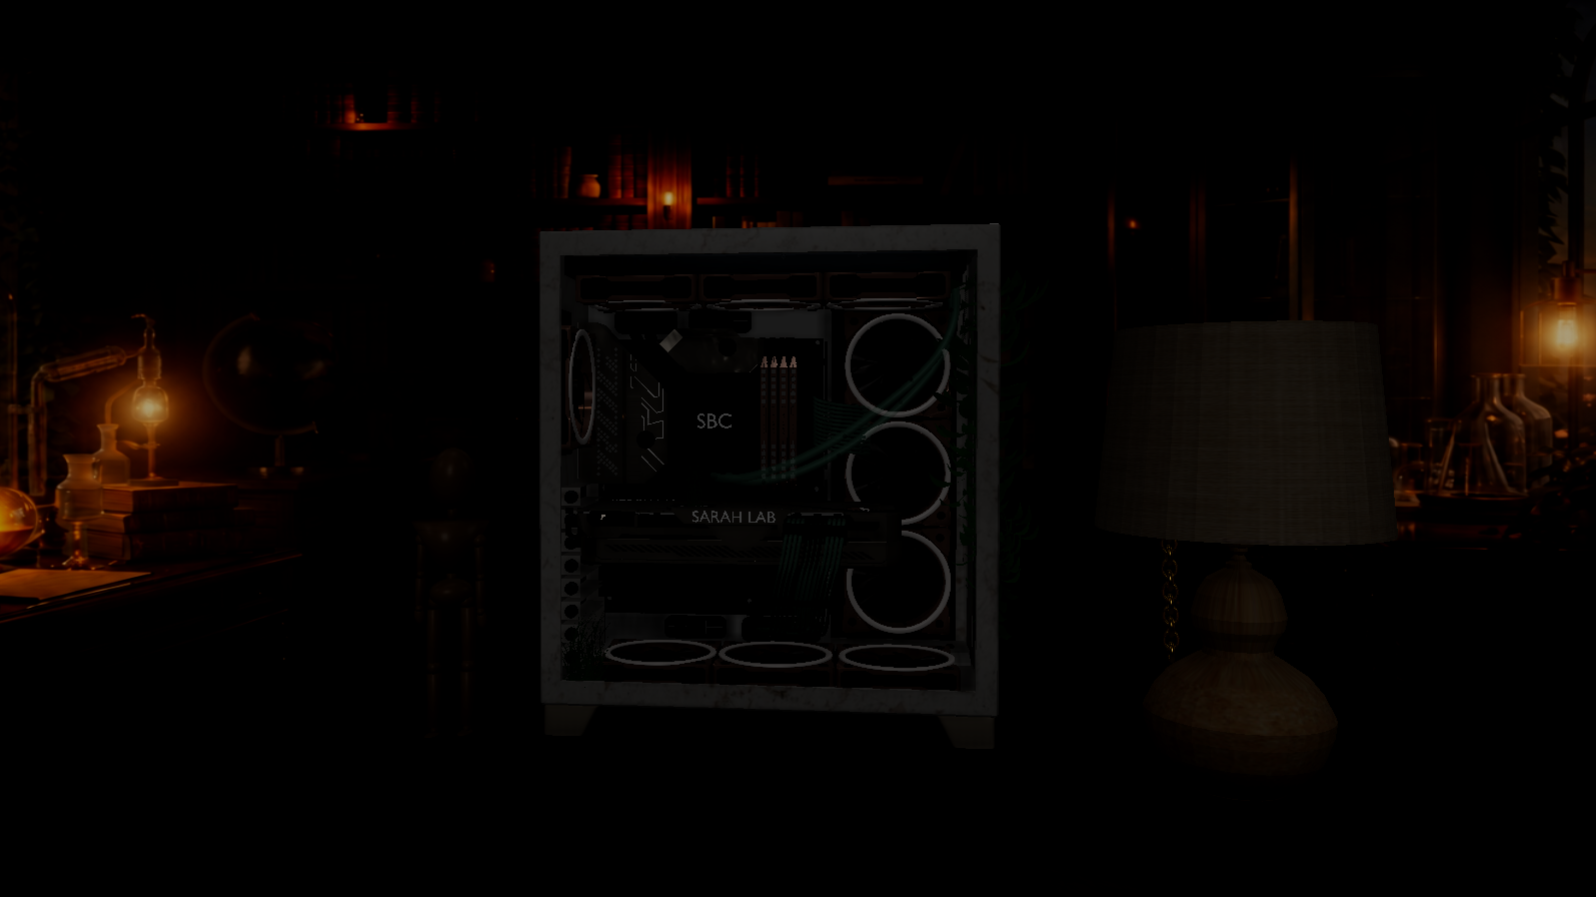
\includegraphics[width=\textwidth]{powered-off scene.png}
        
        \smallskip
        \textbf{(a)} Initial dark state
    \end{minipage}
    \hfill

    \begin{minipage}[t]{0.47\textwidth}
        \centering
        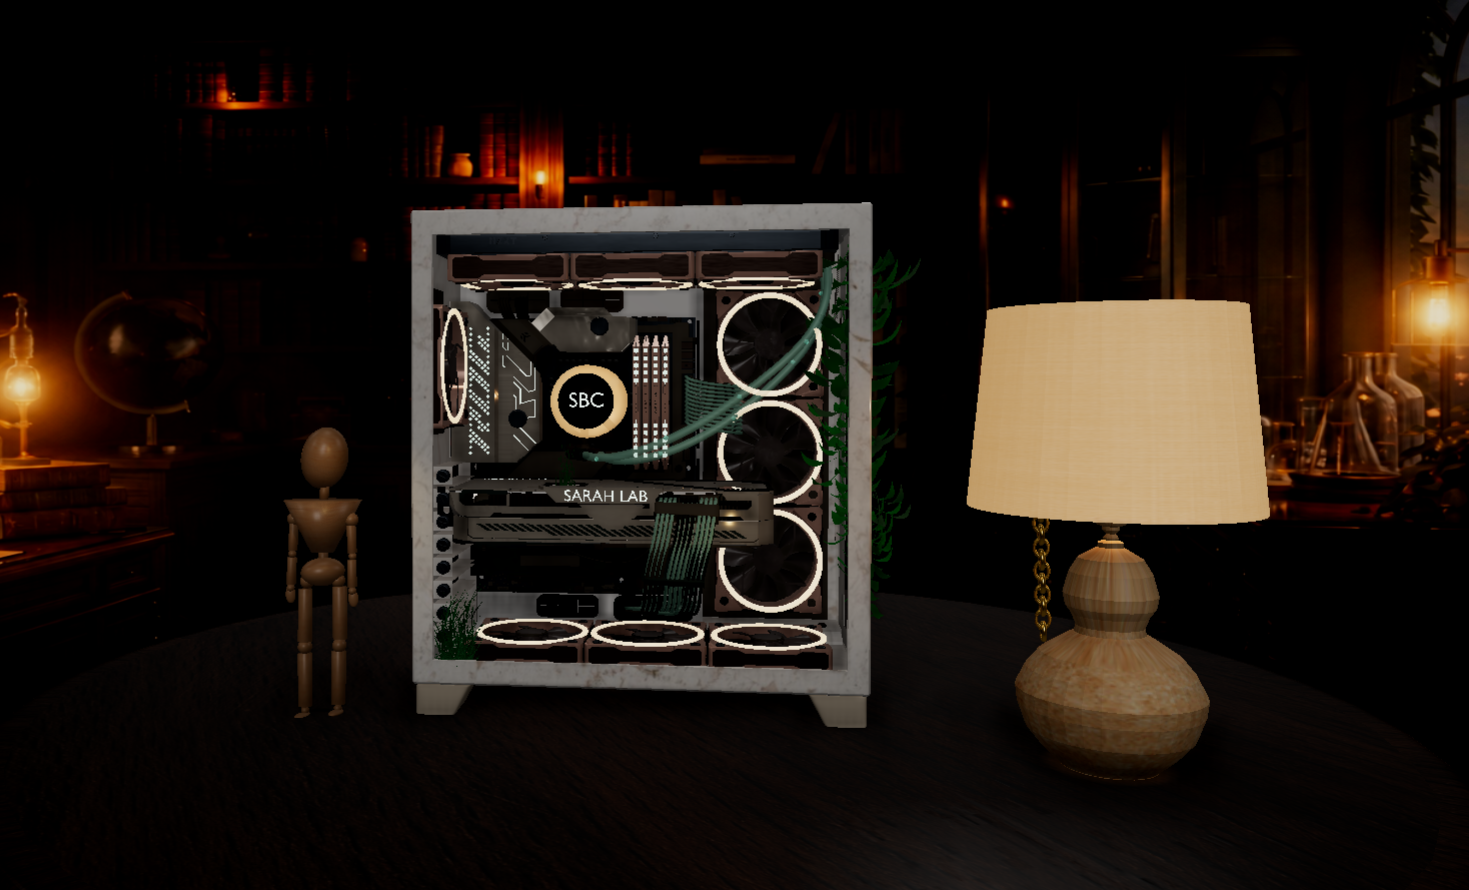
\includegraphics[width=\textwidth]{powered-on scene.png}
        
        \smallskip
        \textbf{(b)} Activated environment
    \end{minipage}
    
    % Didascalia principale della figura
    \caption{Visual state of the environment before and after the lamp-chain interaction.}
    \label{fig:power-state-comparison}
\end{figure}

\subsection{Camera Navigation}

The scene is observed through a perspective camera with a vertical field
of view of \(45^\circ\), an aspect ratio derived from the viewport and a
clipping range from \(0.1\) to \(100\) scene units.

Under perspective projection, points farther from the camera appear
smaller after the homogeneous division. The final clip-space position is
obtained by applying the model, view and projection matrices:

\[
\mathbf{p}_{\mathrm{clip}}
=
\mathbf{P}
\mathbf{V}
\mathbf{M}
\mathbf{p}_{\mathrm{local}}.
\]

The camera initially uses the \texttt{LAMP} preset, directing the user
towards the first interaction. After the computer is activated, the
camera moves to the \texttt{DEFAULT} viewpoint, where the complete case,
Dummy and main environment are visible.

Each clickable portfolio component is associated with a dedicated camera
preset. A preset contains both a camera position and an
\texttt{OrbitControls} target. The two values are animated
simultaneously through GSAP so that the camera translates while also
changing its viewing direction.

\begin{table}[ht]
    \centering
    \small
    \setlength{\tabcolsep}{7pt}
    \renewcommand{\arraystretch}{1.2}

    \begin{tabularx}{\textwidth}{
        @{}
        >{\bfseries\raggedright\arraybackslash}p{0.25\textwidth}
        >{\raggedright\arraybackslash}X
        >{\centering\arraybackslash}p{0.14\textwidth}
        @{}
    }
        \toprule
        Preset & Purpose & Duration \\
        \midrule

        \texttt{LAMP}
        &
        Initial close view of the lamp and chain.
        &
        \(1.6\) s
        \\

        \texttt{DEFAULT}
        &
        Main overview of the complete portfolio environment.
        &
        \(2.4\) s
        \\

        Section presets
        &
        Close views of Dummy, CPU, GPU, RAM, fans and cables.
        &
        \(1.2\) s
        \\

        \bottomrule
    \end{tabularx}

    \caption{Main categories of camera presets.}
    \label{tab:camera-preset-types}
\end{table}

Transitions use a \texttt{sine.inOut} easing function. The controls are
temporarily disabled during movement, preventing user input from
conflicting with the active interpolation. Existing tweens are cancelled
before a new transition begins, and a numerical transition identifier
prevents callbacks from an obsolete animation from changing the current
state.

Outside portfolio panels, \texttt{OrbitControls} allow the user to
rotate, pan and zoom. Damping smooths pointer input, while minimum and
maximum camera distances and polar-angle limits prevent the camera from
moving too close to the assets or below the main table composition.

When a section transition finishes, free camera controls remain disabled
until the corresponding panel is closed. The camera then returns to the
main viewpoint and the controls are enabled again.

\subsection{Raycasting and Interaction State}

Three-dimensional selection is implemented with a
\texttt{THREE.Raycaster}. Pointer coordinates expressed in screen pixels
are first converted into normalised device coordinates:

\[
x_{\mathrm{ndc}} = 2\frac{x}{w}-1,
\qquad
y_{\mathrm{ndc}} = 1-2\frac{y}{h},
\]

where \(w\) and \(h\) are the viewport dimensions. The raycaster then
constructs a ray starting from the camera and passing through the
corresponding point on the projection plane.

The raycaster does not test every visible triangle in the scene. It is
restricted to layer \(1\), which contains only the dedicated
\texttt{CLICK\_} proxy objects. These simplified targets make selection
more reliable and reduce the number of objects evaluated by the
intersection test.

When the pointer is over an actionable target, a CSS class is applied to
the document body to provide cursor feedback. A target is considered
actionable only when its operation is allowed by the current global
interaction state.

The state manager defines four stable or temporary states:

\begin{table}[ht]
    \centering
    \small
    \setlength{\tabcolsep}{7pt}
    \renewcommand{\arraystretch}{1.22}

    \begin{tabularx}{\textwidth}{
        @{}
        >{\bfseries\raggedright\arraybackslash}p{0.24\textwidth}
        >{\raggedright\arraybackslash}X
        @{}
    }
        \toprule
        State & Meaning \\
        \midrule

        \texttt{DARK}
        &
        The system is powered off. Only the lamp-chain interaction is
        available.
        \\

        \texttt{READY}
        &
        The system is powered on and a portfolio component can be
        selected.
        \\

        \texttt{TRANSITIONING}
        &
        A power or camera transition is in progress. Conflicting
        interactions are rejected.
        \\

        \texttt{SECTION\_OPEN}
        &
        A portfolio panel is open and the scene cannot start another
        section interaction.
        \\

        \bottomrule
    \end{tabularx}

    \caption{Global interaction states.}
    \label{tab:interaction-states}
\end{table}

Temporary operations also register named transition locks, such as
\texttt{power}, \texttt{camera:section} and
\texttt{camera:main}. The state returns to a stable value only after all
active locks have been completed. This prevents race conditions between
power transitions, camera movements and panel operations.

Clicking the chain begins a power transition, triggers the chain
animation and, when switching on, moves the camera towards the main case.
Clicking a portfolio target begins a section-camera transition, opens the
associated panel and moves to the corresponding preset. Selecting Dummy
also starts the greeting animation.

Clicks originating inside the HTML panel are ignored by the scene
raycaster. This separation prevents buttons, links and panel navigation
from unintentionally activating three-dimensional targets behind the
interface.

\begin{figure}[H] 
    \centering
    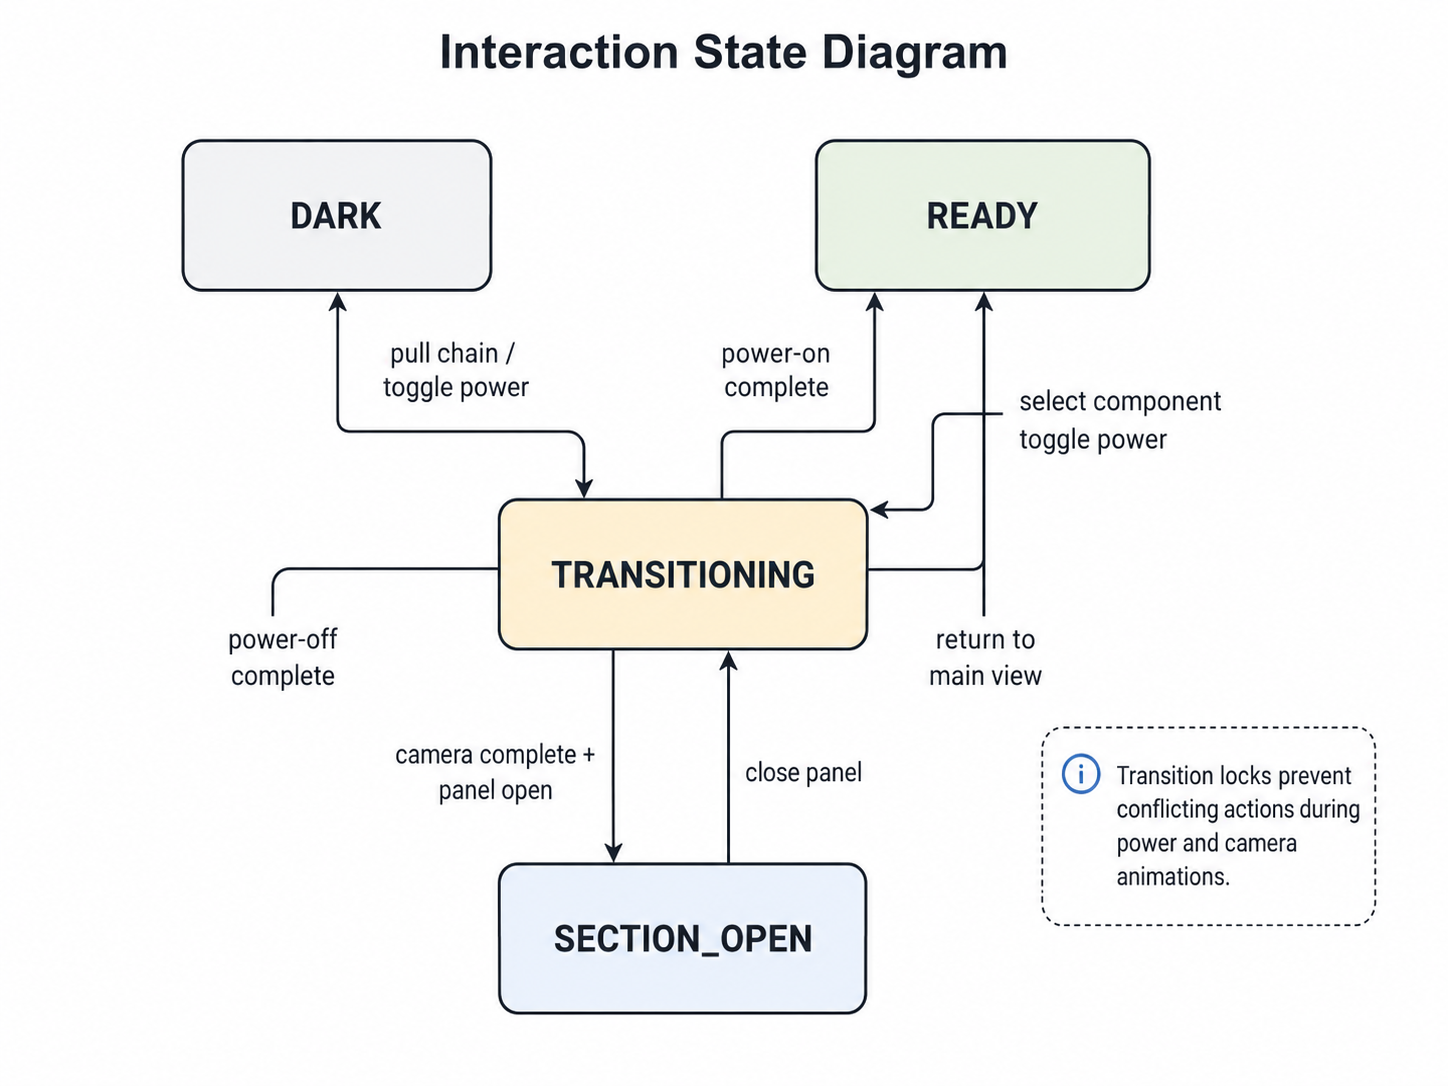
\includegraphics[width=0.8\textwidth]{interaction-state.png}
    \caption{Interaction-state transitions produced by the lamp, camera and portfolio panels.}
\end{figure}


\subsection{Programmatic Animations}

All scene animations are calculated in JavaScript during the render
loop. No animation clips are imported from Blender. Each controller
receives the frame delta and updates the relevant transforms, geometry
or material properties.

\begin{table}[ht]
    \centering
    \footnotesize
    \setlength{\tabcolsep}{5pt}
    \renewcommand{\arraystretch}{1.2}

    \begin{tabularx}{\textwidth}{
        @{}
        >{\bfseries\raggedright\arraybackslash}p{0.20\textwidth}
        >{\raggedright\arraybackslash}p{0.25\textwidth}
        >{\raggedright\arraybackslash}X
        @{}
    }
        \toprule
        Animation & Technique & Behaviour \\
        \midrule

        Dummy idle
        &
        Clamped targets and linear interpolation
        &
        Body, neck and head gradually follow the pointer with different
        amplitudes.
        \\

        Dummy greeting
        &
        Hierarchical rotations, smoothstep and sine waves
        &
        The right arm rises, bends and waves before returning to its
        neutral pose.
        \\

        Lamp chain
        &
        Local translation and vertex deformation
        &
        The chain moves down, remains briefly extended and returns while
        its free end oscillates.
        \\

        Fans
        &
        Time-based local rotation
        &
        Rotors accelerate smoothly to their target speed and decelerate
        after power-off.
        \\

        Tube flow
        &
        Catmull--Rom curves and procedural spheres
        &
        Emissive particles move along sampled cooling-tube paths.
        \\

        LEDs
        &
        Emissive-intensity interpolation
        &
        Case lights follow the powered state; selected fan lights use a
        restrained breathing cycle.
        \\

        Camera
        &
        GSAP interpolation
        &
        Camera position and viewing target move together between
        predefined viewpoints.
        \\

        \bottomrule
    \end{tabularx}

    \caption{Programmatic animation systems implemented in the project.}
    \label{tab:programmatic-animations}
\end{table}

\subsubsection{Dummy idle and greeting}

During the idle state, the pointer position is normalised and used to
compute bounded target rotations. The head receives the largest motion,
the neck a smaller contribution and the body the smallest one. Repeated
linear interpolation produces a delayed response that suggests attention
without abrupt movement.

The greeting lasts approximately \(2.6\) seconds. A smoothstep envelope
raises and lowers the arm, while a sine wave controls the oscillation of
the forearm. The wrist receives a smaller secondary oscillation. At the
end of the animation, the original local rotations are restored.

\subsubsection{Chain deformation}

The chain animation contains three phases: \(0.45\) seconds of downward
movement, a \(1.0\)-second hold and \(0.5\) seconds of return. Both the
visible chain and its invisible proxy follow the same local displacement.

The visible mesh is also deformed by modifying its vertex-position
buffer. Flexibility increases quadratically with distance from the fixed
upper end, and a delayed sine phase creates a travelling oscillation.
After updating the positions, the vertex normals are recomputed. The
original buffer is restored when the animation ends.

\subsubsection{Fan motion}

Each fan rotor is associated with a local axis and a small speed
multiplier. The animator does not switch immediately between zero and
full speed. Instead, the current angular velocity approaches the target
using a fixed acceleration, producing gradual start-up and shutdown.

The angular update is proportional to the frame delta:

\[
\Delta \theta
=
\omega\,m\,\Delta t,
\]

where \(\omega\) is the current speed and \(m\) is the rotor-specific
multiplier. This makes the rotation approximately independent of the
display refresh rate.

\subsubsection{Tube flow}

The two main front tubes are represented by centripetal
\texttt{CatmullRomCurve3} paths sampled from the GLB geometry. Four
procedural spheres are distributed along each curve. Their position is
calculated from

\[
t = (vT + o) \bmod 1,
\]

where \(v\) is the path speed, \(T\) is elapsed time and \(o\) is the
particle offset.

Using centripetal Catmull--Rom interpolation reduces overshooting near
sharp changes of direction. The small auxiliary-tube paths are retained
in the code but disabled in the final configuration.

\subsection{Rendering and Post-Processing}

The renderer uses \texttt{WebGLRenderer} with antialiasing and a
high-performance GPU preference. Output colours are encoded in the sRGB
colour space, while \texttt{ACESFilmicToneMapping} maps high-dynamic-range
lighting values into the displayable range. Exposure changes continuously
with the powered state.

Shadow mapping is enabled with \texttt{PCFShadowMap}. Shadow casting is
restricted to lights and meshes for which it contributes visibly to the
scene. Transparent objects, click proxies, LED surfaces, tube particles
and other decorative elements do not cast shadows.

The post-processing pipeline uses two composers. The first composer
renders only objects assigned to the dedicated bloom layer. During this
pass, non-bloom objects are temporarily replaced by black materials.
For meshes containing multiple material slots, only the slots identified
as LED materials remain visible.

The resulting bloom texture is then combined with the normal scene in
the final composer. The complete order is:

\begin{enumerate}
    \item render the selective bloom layer;
    \item restore the original scene materials and background;
    \item render the normal scene;
    \item optionally apply screen-space ambient occlusion;
    \item add the selective bloom texture;
    \item apply the cinematic finishing shader;
    \item convert the result through \texttt{OutputPass}.
\end{enumerate}

Selective bloom avoids applying a glow to the entire scene. Only the
computer LEDs and explicitly assigned luminous details contribute to the
effect, preserving the readability of the marble, plants, table and
Dummy.

The screen-space ambient-occlusion pass estimates local occlusion from
the depth and normal buffers. It reinforces contact between nearby
surfaces and makes the dense internal components easier to distinguish.
The pass is rendered at half the viewport resolution to reduce its
performance cost. Procedural elements marked as decorative, including
Dummy's contact-shadow plane, are temporarily excluded from the pass.

The final custom shader applies a subtle vignette, contrast adjustment,
cooler shadows and warmer highlights. It also contains support for
screen-space glows aligned with the background lamps, although their
current configured contribution is disabled.

If the browser cannot create a WebGL context, the renderer hides the
canvas and replaces the loading screen with a fallback message. The
application therefore fails explicitly rather than leaving the user on
an indefinitely loading page.

\begin{figure}[ht]
    \centering
    
    \begin{minipage}[t]{0.47\textwidth}
        \centering
        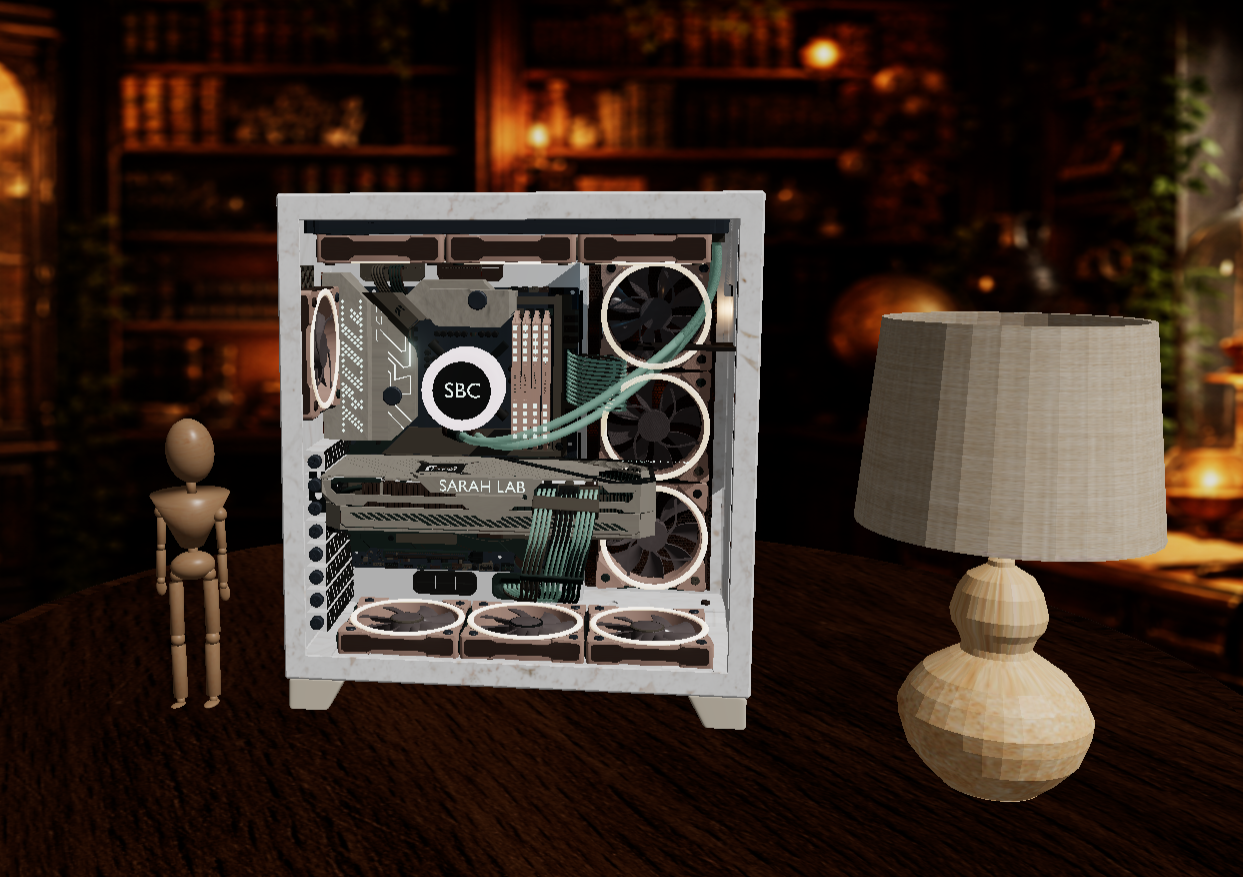
\includegraphics[width=\textwidth]{before-post-processing.png}
        
        \smallskip
        \textbf{(a)} Before post processing
    \end{minipage}
    \hfill
    \begin{minipage}[t]{0.47\textwidth}
        \centering
        
        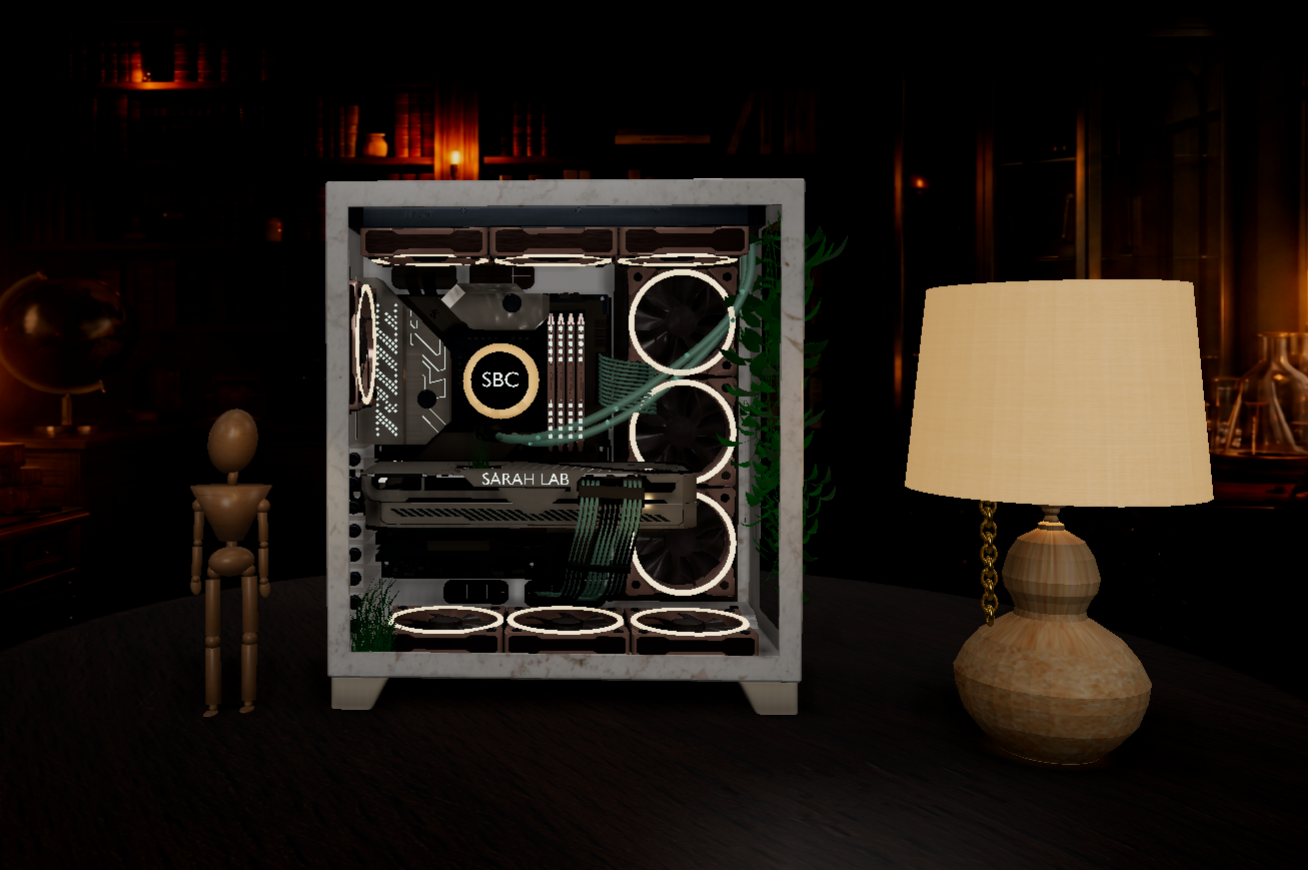
\includegraphics[width=\textwidth]{after-post-processing.png}
        
        \smallskip
        \textbf{(b)} After post processing
    \end{minipage}
    
    \caption{Comparison between the base scene rendering and the final result after applying the post-processing pipeline.}
    \label{fig:post-processing-comparison}
\end{figure}


\subsection{Performance Optimisation}

The original scene used several high-resolution PBR texture sets. The
selected source textures occupied approximately \(505\,\mathrm{MiB}\),
which produced long loading times and excessive GPU-memory consumption
for a web application.

A dedicated optimisation script defines a maximum resolution and output
quality for each map and invokes a Python routine based on Pillow.
Different maps are reduced according to their visual role.

\begin{table}[ht]
    \centering
    \small
    \setlength{\tabcolsep}{6pt}
    \renewcommand{\arraystretch}{1.2}

    \begin{tabularx}{\textwidth}{
        @{}
        >{\bfseries\raggedright\arraybackslash}p{0.24\textwidth}
        >{\centering\arraybackslash}p{0.18\textwidth}
        >{\centering\arraybackslash}p{0.18\textwidth}
        >{\raggedright\arraybackslash}X
        @{}
    }
        \toprule
        Map category & Typical source & Typical output & Rationale \\
        \midrule

        Main colour maps
        &
        \(4096^2\)
        &
        \(2048^2\)
        &
        Preserves visible detail on the case and table.
        \\

        Other colour maps
        &
        \(4096^2\)
        &
        \(1024^2\)
        &
        Sufficient for smaller components and Dummy.
        \\

        Normal maps
        &
        \(2048^2\)--\(4096^2\)
        &
        \(1024^2\)
        &
        Retains surface detail while reducing memory use.
        \\

        Roughness and metalness
        &
        \(2048^2\)--\(4096^2\)
        &
        \(512^2\)
        &
        These maps generally contain lower-frequency information.
        \\

        \bottomrule
    \end{tabularx}

    \caption{Resolution strategy used for texture optimisation.}
    \label{tab:texture-optimisation-strategy}
\end{table}

The resulting optimised set occupies approximately
\(4.7\,\mathrm{MiB}\), corresponding to a reduction of \(99.1\%\) for
the selected files. The optimised versions are stored under
\texttt{public/textures\_optimized} and are the only versions loaded by
the runtime material system.

Additional rendering optimisations include:

\begin{itemize}
    \item limiting the renderer pixel ratio to \(1.5\);
    \item calculating SSAO at half resolution;
    \item restricting bloom to a dedicated layer;
    \item disabling shadows on transparent and decorative elements;
    \item using only the two confirmed large cooling-tube paths;
    \item sharing procedural geometries where possible;
    \item clamping unusually large frame deltas in the animation systems;
    \item building and minifying the application through Vite.
\end{itemize}

The application is deployed through a GitHub Actions workflow. Every
push to the \texttt{main} branch can install the dependencies with
\texttt{npm ci}, execute the production Vite build, upload the
\texttt{dist} directory and publish it through GitHub Pages. The Vite
configuration derives the repository name from the
\texttt{GITHUB\_REPOSITORY} environment variable and uses it as the base
path for production assets.

\section{User Interaction}

\subsection{Starting the Application}

After opening the application, the user first sees the loading interface.
When the GLB has been processed, the loading screen fades away and the
camera remains focused on the lamp. A temporary guidance message asks
the user to pull the chain.

At this stage, the global state is \texttt{DARK}. Portfolio components
cannot yet be opened. Moving the pointer over the chain changes the
cursor feedback, indicating that the object is interactive.

Clicking the chain performs three coordinated actions:

\begin{enumerate}
    \item the visible chain is pulled and deformed;
    \item the lamp and computer begin their power transition;
    \item the camera moves from the lamp to the main case viewpoint.
\end{enumerate}

Once the transition has finished, the application enters the
\texttt{READY} state. The fans rotate, the tube-flow particles move and
the case LEDs become visible.

\subsection{Exploring the Scene}

In the main view, the user can:

\begin{itemize}
    \item drag to rotate the camera;
    \item drag using the appropriate pointer control to pan;
    \item use the mouse wheel or trackpad to zoom;
    \item select Dummy or a computer component;
    \item press the reset-view button to return to the case overview.
\end{itemize}

Camera movement is constrained to preserve the intended composition.
The user cannot move below the table or zoom indefinitely through the
models.

The interactive mapping is summarised in
Table~\ref{tab:portfolio-interaction-map}.

\begin{table}[ht]
    \centering
    \small
    \setlength{\tabcolsep}{6pt}
    \renewcommand{\arraystretch}{1.2}

    \begin{tabularx}{\textwidth}{
        @{}
        >{\bfseries\raggedright\arraybackslash}p{0.20\textwidth}
        >{\raggedright\arraybackslash}p{0.25\textwidth}
        >{\raggedright\arraybackslash}X
        @{}
    }
        \toprule
        Scene element & Target & Portfolio content \\
        \midrule

        Dummy
        &
        \texttt{CLICK\_DUMMY}
        &
        Contact links and information about the project.
        \\

        CPU
        &
        \texttt{CLICK\_CPU}
        &
        About Me.
        \\

        GPU
        &
        \texttt{CLICK\_GPU}
        &
        Academic and personal projects.
        \\

        RAM
        &
        \texttt{CLICK\_RAM}
        &
        Academic background.
        \\

        Fans
        &
        \texttt{CLICK\_FANS}
        &
        Work experience.
        \\

        Cooling cables
        &
        \texttt{CLICK\_CABLES}
        &
        Hobbies and interests.
        \\

        Lamp chain
        &
        \texttt{CLICK\_CHAIN}
        &
        Turns the system on or off.
        \\

        \bottomrule
    \end{tabularx}

    \caption{Mapping between three-dimensional targets and portfolio sections.}
    \label{tab:portfolio-interaction-map}
\end{table}

\subsection{Opening and Closing a Section}

Selecting a valid component starts a controlled camera movement towards
the object and opens the associated panel. While the transition is in
progress, additional scene interactions are disabled.

When the camera reaches the selected component, free controls remain
disabled and the state changes to \texttt{SECTION\_OPEN}. The user can
then read and navigate the HTML content without the scene moving behind
the panel.

The panel is closed through its dedicated close button. This starts a
return transition to the main view. After the camera reaches the default
position, the application re-enters the \texttt{READY} state and camera
controls become available again.

The lamp cannot be toggled while a section is open or while another
transition is active. This restriction prevents the visual power state,
camera and interface from becoming inconsistent.

\subsection{Guidance Messages}

The guidance overlay provides short contextual instructions. The initial
message explains the lamp-chain interaction. After the system is
activated and the camera reaches the main view, a second message explains
component selection, dragging and zooming.

The overlay also monitors pointer, touch, wheel, keyboard and click
activity. After approximately \(30\) seconds of inactivity, it can
display one contextual reminder:

\begin{itemize}
    \item in the powered-off state, it suggests pulling the lamp chain;
    \item in the powered-on state, it suggests selecting Dummy or a
    component.
\end{itemize}

A reminder is shown only when the model has loaded, no panel is open, no
transition is active and camera controls are enabled.

\section{Portfolio Interface}

The three-dimensional environment is combined with an HTML interface
used to present the actual portfolio information. Keeping text in the
DOM rather than rendering it as three-dimensional geometry improves
readability, accessibility, responsive layout and link interaction.

\subsection{Section Panel}

The main interface is a panel positioned on the right side of the
viewport. It slides into view when a portfolio section is selected and
contains a title, content area, navigation controls and close button.

The panel supports both simple and structured pages. Simple sections
display a title and paragraph, while more complex sections generate
specialised views from the data stored in
\texttt{portfolioSections.js}.

The content data is therefore separated from the presentation logic.
Updating a project description or adding an academic entry does not
require modifying the Three.js interaction system.

\subsection{Dummy and About Me}

Dummy contains two pages. The first provides contact links for email,
LinkedIn, GitHub and Instagram. The icons are generated from SVG paths
and include descriptive labels.

The second page introduces the project and explains its connection
between engineering and illustration. Previous and next controls are
shown only when another page is available.

The CPU opens the About Me section, which presents a concise professional
summary focused on Artificial Intelligence, Robotics, computer graphics
and interactive application development.

\subsection{Academic Background}

The RAM section uses an accessible tabbed interface for the master's
degree, bachelor's degree and Erasmus experience. Each tab is connected
to a corresponding panel through ARIA attributes.

The tabs can be navigated with the mouse or keyboard. The supported keys
are:

\begin{itemize}
    \item left and right arrows to move between entries;
    \item \texttt{Home} to select the first entry;
    \item \texttt{End} to select the final entry.
\end{itemize}

Focus is moved together with the selected tab, and inactive panels are
hidden from the layout.

\subsection{Projects}

The GPU section initially displays an ordered project index. Each entry
contains a number, title, category and year. Selecting an entry replaces
the index with a detailed project view.

Project details can contain:

\begin{itemize}
    \item academic or personal context;
    \item role;
    \item project description;
    \item principal contributions;
    \item quantitative results;
    \item technologies.
\end{itemize}

A dedicated back button returns to the index and restores focus to the
previously selected project. This creates an internal navigation system
without leaving the portfolio panel.

\subsection{Work Experience and Interests}

The fan section follows a similar index-and-detail structure for
professional experiences. Each entry can include company, role, period,
location, summary, responsibilities and technologies.

The cable section presents hobbies and interests in a simpler textual
format. Its panel style disables the expensive backdrop filter to avoid
interfering with the smooth fan animation visible behind it.

\subsection{Responsive and Accessible Behaviour}

The interface uses semantic buttons, headings, lists, tabs and links.
The guidance overlay has \texttt{role="status"} and an
\texttt{aria-live} region, allowing non-disruptive announcements by
assistive technologies.

The panel and guidance overlay adapt to narrow screens through CSS media
queries. Structured sections can scroll vertically when their content
exceeds the available viewport height. The stylesheet also respects the
\texttt{prefers-reduced-motion} media query for guidance transitions.

The three-dimensional targets themselves remain primarily pointer-based.
Keyboard accessibility is stronger within the DOM interface than in the
scene-selection stage, which is discussed among the future
improvements.

\begin{figure}[ht]
    \centering
    
\includegraphics[width=0.8\textwidth]{panel-layouts.png}
    \caption{Examples of the HTML portfolio interface.}
    \label{fig:panel-layouts}
\end{figure}


\section{Development and Debugging Tools}

\subsection{Debug Mode}

Development diagnostics are isolated in the
\texttt{DebugUtils} class. They are enabled by adding
\texttt{?debug=1} to the application URL. When debug mode is disabled,
the additional click and keyboard listeners are not registered.

After the GLB has loaded, the utility can print the Dummy hierarchy,
inspect material properties and analyse the complete model. The model
diagnostics include:

\begin{itemize}
    \item number of meshes;
    \item approximate triangle count;
    \item number of distinct material instances;
    \item the heaviest meshes by triangle count;
    \item repeated material names;
    \item textures with large dimensions;
    \item shadow and visibility flags.
\end{itemize}

Clicking a visible mesh in debug mode prints its complete ancestor chain,
making it easier to determine how an imported Blender object is
represented in the Three.js scene graph.

\subsection{Camera Calibration}

Camera presets were calibrated through dedicated debug controls. After
selecting a \texttt{CLICK\_} target, the utility stores it as the current
calibration object. Its world-space bounding box is used to calculate a
suitable camera target and distance.

\begin{table}[ht]
    \centering
    \small
    \setlength{\tabcolsep}{7pt}
    \renewcommand{\arraystretch}{1.2}

    \begin{tabularx}{\textwidth}{
        @{}
        >{\bfseries\centering\arraybackslash}p{0.15\textwidth}
        >{\raggedright\arraybackslash}X
        @{}
    }
        \toprule
        Key & Debug action \\
        \midrule

        \texttt{F}
        &
        Frames the currently selected calibration target.
        \\

        \texttt{P}
        &
        Prints the current camera position and controls target in a
        preset-compatible format.
        \\

        \texttt{D}
        &
        Prints the current camera values using the
        \texttt{DEFAULT} preset name.
        \\

        \texttt{0}
        &
        Moves the camera back to the default viewpoint when interactions
        are not locked.
        \\

        \bottomrule
    \end{tabularx}

    \caption{Keyboard commands available in debug mode.}
    \label{tab:debug-keys}
\end{table}

The current \texttt{Experience} instance is also exposed through
\texttt{window.\_\_INTERACTIVE\_CV\_\_} when Vite is running in
development mode. The tube-flow controller provides additional console
helpers for inspecting the animator and comparing sampled curve
positions with GLB meshes.

\subsection{Build and Deployment}

The local development workflow uses the following npm commands:

\begin{verbatim}
npm run dev
npm run build
npm run preview
\end{verbatim}

The development server provides ES-module loading and fast updates.
The production command creates the optimised static files in the
\texttt{dist} directory, while the preview command serves the final
build locally.

Deployment is automated through GitHub Actions. The workflow runs on
Ubuntu with Node.js 22, installs exact dependencies through
\texttt{npm ci}, builds the application and uploads the generated
directory to GitHub Pages.

\begin{figure}[H]
    \centering
    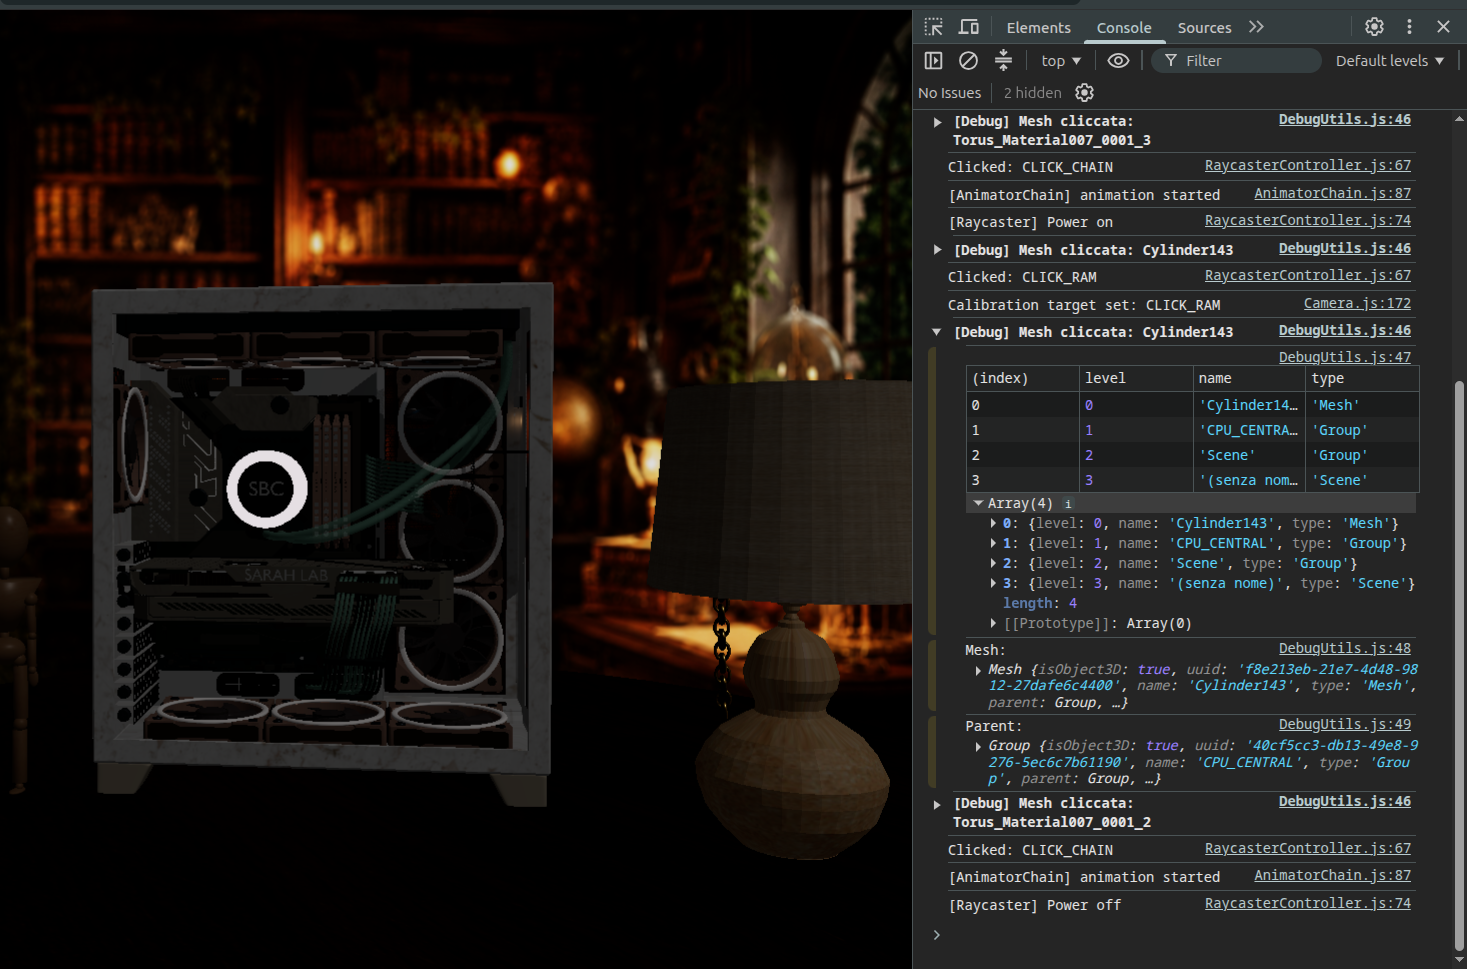
\includegraphics[width=0.8\textwidth]{debug-tools.png}
    \caption{Example of the development diagnostics used during scene
    calibration and optimisation.}
    \label{fig:debug-tools}
\end{figure}


\section{Known Limitations and Future Improvements}

The final application satisfies the principal functional requirements,
but several aspects could be improved in a future version.

\begin{table}[ht]
    \centering
    \footnotesize
    \setlength{\tabcolsep}{5pt}
    \renewcommand{\arraystretch}{1.2}

    \begin{tabularx}{\textwidth}{
        @{}
        >{\bfseries\raggedright\arraybackslash}p{0.22\textwidth}
        >{\raggedright\arraybackslash}p{0.34\textwidth}
        >{\raggedright\arraybackslash}X
        @{}
    }
        \toprule
        Area & Current limitation & Possible improvement \\
        \midrule

        Initial loading
        &
        The scene is distributed as one relatively large GLB and is
        configured only after the complete file has loaded.
        &
        Divide the environment into independently loaded assets or
        introduce progressive loading.
        \\

        Rendering cost
        &
        Selective bloom, SSAO, shadows and a detailed GLB can be
        demanding on integrated or mobile GPUs.
        &
        Add automatic quality levels that reduce pixel ratio, disable
        SSAO or simplify shadows on slower devices.
        \\

        Desktop-first controls
        &
        The visual configuration and camera navigation were primarily
        calibrated for desktop displays.
        &
        Create dedicated mobile camera presets and touch-oriented
        interaction affordances.
        \\

        Naming dependency
        &
        Runtime discovery relies on semantic Blender names such as
        \texttt{CLICK\_*}, \texttt{FAN\_ROT\_*} and
        \texttt{Dummy\_*}.
        &
        Export explicit metadata through glTF extras or maintain a
        central validated asset manifest.
        \\

        Tube animation
        &
        Only the two principal front tubes are enabled; the smaller
        predefined paths remain disabled.
        &
        Calibrate the remaining paths and use instancing when adding
        more particles.
        \\

        Frame-rate response
        &
        Some idle movements use fixed interpolation factors rather than
        fully time-correct exponential damping.
        &
        Express every smoothing factor as a function of frame delta.
        \\

        Scene accessibility
        &
        The HTML panels support keyboard interaction, but the initial
        three-dimensional target selection is pointer-oriented.
        &
        Add a keyboard-accessible component menu linked to the same
        camera and panel actions.
        \\

        Dependency cleanup
        &
        \texttt{@tweenjs/tween.js} remains installed although the final
        camera system uses GSAP.
        &
        Remove unused dependencies before the final production release.
        \\

        Cinematic introduction
        &
        Support exists for an automatic introduction, but it is disabled
        to avoid a visible flicker during the first load.
        &
        Coordinate the introduction with an explicit asset-preloading
        and rendering-ready state.
        \\

        \bottomrule
    \end{tabularx}

    \caption{Current limitations and possible future developments.}
    \label{tab:future-improvements}
\end{table}

Further development could also include sound effects for the lamp, fans
and background environment, a reduced-motion option affecting all
three-dimensional animations, and a richer visual indication of the
currently focused component.

Despite these limitations, the project demonstrates how a conventional
portfolio can be transformed into an interactive real-time experience.
The final application combines an authored three-dimensional scene,
hierarchical modelling, physically based materials, multiple lighting
systems, GPU post-processing, programmatic animation and a structured
web interface within a single narrative environment.


\clearpage
\begin{thebibliography}{99}

\bibitem{project-repository}
Sara Cristina Basco,
\textit{Inside My System -- Source Repository},
Sapienza Interactive Graphics Course.
\url{https://github.com/SapienzaInteractiveGraphicsCourse/final-project-karu_akai}

\bibitem{threejs}
Three.js Authors,
\textit{Three.js Documentation}.
\url{https://threejs.org/docs/}

\bibitem{gltf-loader}
Three.js Authors,
\textit{GLTFLoader}.
\url{https://threejs.org/docs/#examples/en/loaders/GLTFLoader}

\bibitem{orbit-controls}
Three.js Authors,
\textit{OrbitControls}.
\url{https://threejs.org/docs/#examples/en/controls/OrbitControls}

\bibitem{three-postprocessing}
Three.js Authors,
\textit{Post-Processing Manual}.
\url{https://threejs.org/manual/en/post-processing.html}

\bibitem{gltf-specification}
Khronos Group,
\textit{glTF 2.0 Specification}.
\url{https://registry.khronos.org/glTF/specs/2.0/glTF-2.0.html}

\bibitem{gsap}
GreenSock,
\textit{GSAP Documentation}.
\url{https://gsap.com/docs/v3/}

\bibitem{vite}
Vite Contributors,
\textit{Vite Documentation}.
\url{https://vite.dev/guide/}

\bibitem{blender}
Blender Foundation,
\textit{Blender}.
\url{https://www.blender.org/}

\bibitem{pillow}
Pillow Contributors,
\textit{Pillow Documentation}.
\url{https://pillow.readthedocs.io/}

\bibitem{ambientcg}
ambientCG,
\textit{Public-Domain PBR Materials}.
\url{https://ambientcg.com/}

\bibitem{simple-icons}
Simple Icons Contributors,
\textit{Simple Icons}.
\url{https://simpleicons.org/}

\bibitem{sketchfab-table}
yryabchenko,
\textit{Table},
Sketchfab.
\url{https://sketchfab.com/3d-models/table-1132fa2850a24917892733566bd68e74}

\bibitem{sketchfab-computer}
Marcseus,
\textit{Gaming Computer},
Sketchfab.
\url{https://sketchfab.com/3d-models/gaming-computer-7cf383ddfe9047f89435b4fc2a6e1053}

\bibitem{cc-by}
Creative Commons,
\textit{Attribution 4.0 International}.
\url{https://creativecommons.org/licenses/by/4.0/}

\bibitem{cc-zero}
Creative Commons,
\textit{CC0 1.0 Universal}.
\url{https://creativecommons.org/publicdomain/zero/1.0/}

\bibitem{github-pages}
GitHub,
\textit{GitHub Pages Documentation}.
\url{https://docs.github.com/en/pages}

\bibitem{course-material}
Marco Schaerf,
\textit{Interactive Graphics Course Materials:
Raster Images, Two- and Three-Dimensional Transformations,
GPU Pipeline and WebGL, Surfaces, Triangular Meshes and GPU Textures},
Sapienza University of Rome, Academic Year 2025--2026.

\end{thebibliography}

\end{document}
